%%
%% This is file `sample-sigplan.tex',
%% generated with the docstrip utility.
%%
%% The original source files were:
%%
%% samples.dtx  (with options: `sigplan')
%% 
%% IMPORTANT NOTICE:
%% 
%% For the copyright see the source file.
%% 
%% Any modified versions of this file must be renamed
%% with new filenames distinct from sample-sigplan.tex.
%% 
%% For distribution of the original source see the terms
%% for copying and modification in the file samples.dtx.
%% 
%% This generated file may be distributed as long as the
%% original source files, as listed above, are part of the
%% same distribution. (The sources need not necessarily be
%% in the same archive or directory.)
%%
%%
%% Commands for TeXCount
%TC:macro \cite [option:text,text]
%TC:macro \citep [option:text,text]
%TC:macro \citet [option:text,text]
%TC:envir table 0 1
%TC:envir table* 0 1
%TC:envir tabular [ignore] word
%TC:envir displaymath 0 word
%TC:envir math 0 word
%TC:envir comment 0 0
%%
%%
%% The first command in your LaTeX source must be the \documentclass command.
\documentclass[sigplan,screen]{acmart}

%%
%% \BibTeX command to typeset BibTeX logo in the docs
\AtBeginDocument{%
  \providecommand\BibTeX{{%
    Bib\TeX}}}

%% Rights management information.  This information is sent to you
%% when you complete the rights form.  These commands have SAMPLE
%% values in them; it is your responsibility as an author to replace
%% the commands and values with those provided to you when you
%% complete the rights form.
\setcopyright{rightsretained}
\copyrightyear{2022}
%\acmYear{2018}
%\acmDOI{XXXXXXX.XXXXXXX}

%% These commands are for a PROCEEDINGS abstract or paper.
%acmConference[Machine Learning for Behavioural Data (CS-421)]{}{12th of June,
 % 2022}{Lausanne, CH}
%\acmPrice{15.00}
%\acmISBN{978-1-4503-XXXX-X/18/06}


%%
%% Submission ID.
%% Use this when submitting an article to a sponsored event. You'll
%% receive a unique submission ID from the organizers
%% of the event, and this ID should be used as the parameter to this command.
%%\acmSubmissionID{123-A56-BU3}

%%
%% For managing citations, it is recommended to use bibliography
%% files in BibTeX format.
%%
%% You can then either use BibTeX with the ACM-Reference-Format style,
%% or BibLaTeX with the acmnumeric or acmauthoryear sytles, that include
%% support for advanced citation of software artefact from the
%% biblatex-software package, also separately available on CTAN.
%%
%% Look at the sample-*-biblatex.tex files for templates showcasing
%% the biblatex styles.
%%

%%
%% The majority of ACM publications use numbered citations and
%% references.  The command \citestyle{authoryear} switches to the
%% "author year" style.
%%
%% If you are preparing content for an event
%% sponsored by ACM SIGGRAPH, you must use the "author year" style of
%% citations and references.
%% Uncommenting
%% the next command will enable that style.
%%\citestyle{acmauthoryear}

\usepackage{csquotes}
\usepackage{subcaption}
\settopmatter{printfolios=true}
%%
%% end of the preamble, start of the body of the document source.
\begin{document}

%%
%% The "title" command has an optional parameter,
%% allowing the author to define a "short title" to be used in page headers.
\title[Do As I Do]{Do as I Do -- Identification of Student Behavioural Patterns to Predict Attainment on an Online Learning Platform}

%%
%% The "author" command and its associated commands are used to define
%% the authors and their affiliations.
%% Of note is the shared affiliation of the first two authors, and the
%% "authornote" and "authornotemark" commands
%% used to denote shared contribution to the research.
\author{Kai Cooper}
\authornote{All authors contributed equally to this research.}
\affiliation{%
  \institution{EPFL, Mathematics (exchange from Imperial College London)}
  \city{Lausanne}
  \state{Vaud}
  \country{Switzerland}
}
\email{kai.cooper@epfl.ch}

\author{Nicolas d'Argenlieu}
\authornotemark[1]
\affiliation{%
  \institution{EPFL, Data Science (Master)}
  \city{Lausanne}
  \state{Vaud}
  \country{Switzerland}}
\email{nicolas.thierrydargenlieu@epfl.ch}

\author{Mar\'ia Isabel Ruiz Mart\'inez}
\authornotemark[1]
\affiliation{%
  \institution{EPFL, Computer Science (exchange from Universidad de Granada)}
  \city{Lausanne}
  \state{Vaud}
  \country{Switzerland}
}
\email{maria.ruizmartinez@epfl.ch}


%%
%% By default, the full list of authors will be used in the page
%% headers. Often, this list is too long, and will overlap
%% other information printed in the page headers. This command allows
%% the author to define a more concise list
%% of authors' names for this purpose.
\renewcommand{\shortauthors}{Cooper et al.}

%%
%% The abstract is a short summary of the work to be presented in the
%% article.
\begin{abstract}
In this report, we present the results of a learning analytics study. The analyzed data is produced by chronologically recorded clickstreams of Swiss secondary school student usage of the online maths and German learning platform Lernnavi. We quantify student behavioural patterns, in particular their regularity, and use these features to predict student attainment on the platform through a supervised learning pipeline. Our results reinforce that regular and persistent usage of the platform leads to better performance, however our models also serve to highlight some of the pitfalls of aiming to study human behaviour through opaque clickstreams. 
\end{abstract}

%%
%% Keywords. The author(s) should pick words that accurately describe
%% the work being presented. Separate the keywords with commas.
\keywords{dataset, regularity, decision trees, random forest classifier, time series classification, support vector, kernel function, silhouette score, prediction, clustering, lernnavi, moocs, education, student attainment}
%% A "teaser" image appears between the author and affiliation
%% information and the body of the document, and typically spans the
%% page.
\begin{teaserfigure}
  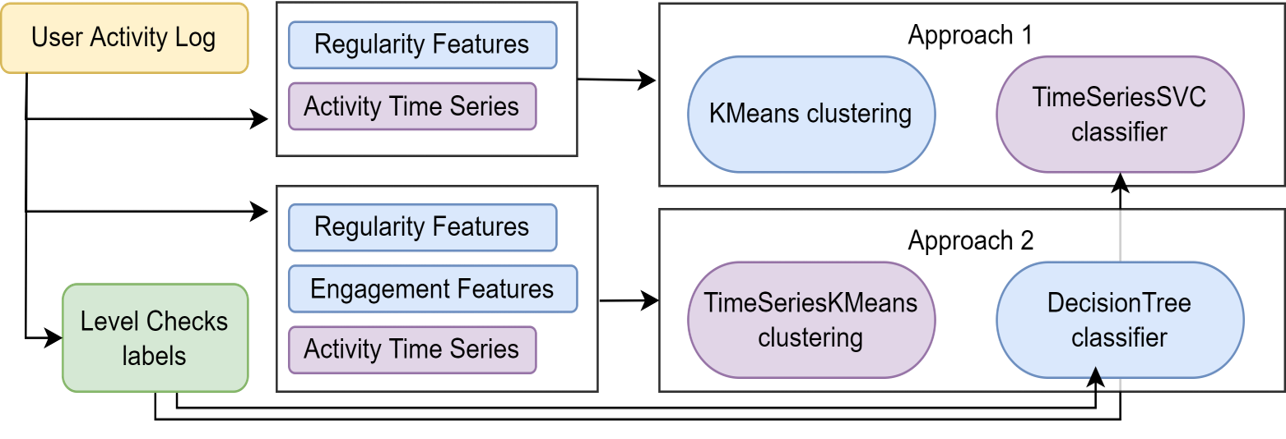
\includegraphics[width=\textwidth]{reports/figures/approaches_schema.png}
  \caption{Overview of the modelling methodology employed in this report.}
  \label{fig:teaser}
\end{teaserfigure}

%%
%% This command processes the author and affiliation and title
%% information and builds the first part of the formatted document.
\maketitle

\section{Introduction}\label{sec:intro}
Improved digital technologies have made online learning formats such as MOOCs and dedicated learning platforms such as Moodle more accessible. Lernnavi is one of these online education platforms, whose primary use is as an accompanying teaching and learning tool in secondary education. They offer maths and German lessons and exercises. Students track their progress through a mastery score updated by so-called \textbf{level checks}, unique to each topic taught on the platform. 

\subsection{Research Question}\label{subsec:researchQ}

Innately, we are all aware of the fact that self-improvement demands commitment. This notion is omnipresent in education and is a persistent device used by educators to encourage learning. Consequently, we anticipate that students who choose (or are perhaps forced) to exhibit regular, recurrent patterns of learning behaviours will experience greater learning gains in the long-run. In this project, we wish to discover if this phenomenon is present within the Lernnavi environment, while going to a step further and identify which specific behaviours \textit{may} lead to higher attainment for a given student. In light of this, we state our research question:

\begin{displayquote}
\textit{Is it possible to identify one or more studying behaviors leading to a significant improvement in level check results?}
\end{displayquote}



\section{Data Description and Exploratory Analysis}\label{sec:data}

%{\color{red}
%\begin{itemize}
    %\item Data description in its \textbf{most raw form}: what the different tables are and their contents (overview); shape of most important datasets.
    %\item Exploratory analysis based on the above.
    %\item Vast majority of students on the platform belong to year groups gymnasium 1, 2 and 3 (the first group the largest)
    %\item 32\% male, 39\% female, 29\% NA, 3\% Prefer to not disclose. 
    %\item Distribution of actions, transactions etc is strongly decaying. (Fewer students do more actions).  
    %\item \textbf{Note: for the above, much has already been done.} 
%\end{itemize}
%}

The educational platform Lernnavi provided us with a series of datasets reflecting the usage of the platform, among which $\texttt{learn\_sessions\_transactions}$, $\texttt{users}$, $\texttt{events}$ and $\texttt{transactions}$ will be used to carry out our research work.

The $\texttt{learn\_sessions\_transactions}$ dataset ($502,921$ rows) contains information about the sessions of the platform. The sessions describe a learn or a level check session started and/or finished by a user and they are sorted chronologically, row by row. Additionally, for each session, there are one or more associated transactions (i.e., answers to tasks in that student's session).

The $\texttt{users}$ dataset ($13,790$ rows) contains demographic information of the users of the educational platform. The $\texttt{events}$ dataset ($3,465,559$ rows) describe the events done by the users in the platform. Finally, the $\texttt{transactions}$ dataset ($800,018$ rows) reflects the multiple user transactions (e.g., answering a question) for each session. The detailed feature description of the datasets is shown in the Tables \ref{tab:learn}, \ref{tab:users}, \ref{tab:events} and \ref{tab:transactions}.

\begin{figure}[h]
    \centering
    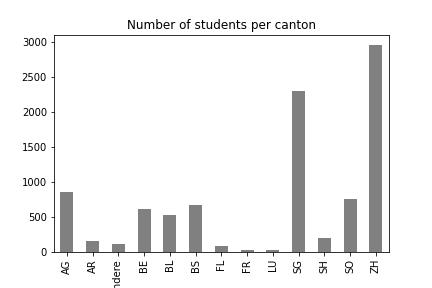
\includegraphics[width=\linewidth]{reports/figures/num_per_canton.jpg}
    \caption{Bar plot of the number of students per canton. Zurich and St. Gallen contain most of the users on the platform.}
    \label{fig:my_label}
\end{figure}

A study on the $\texttt{gender}$, $\texttt{canton}$ and $\texttt{class\_level}$ of the users of the platform was also performed. We remark that there is a geographical element to the data (shown in Figures \ref{fig:my_label} and \ref{fig:cantonal_representation}), and this is important because it might introduce mixed effects between the groups of students by region. Consequently we investigated to some degree the cantonal representation within the dataset and how activity on the platform varied with location. At this stage it is quite preliminary is essentially an aperçu into what additional features we may need to include in the model for more accurate results (find more details in the associated notebook).

\begin{figure}[h]
    \centering
    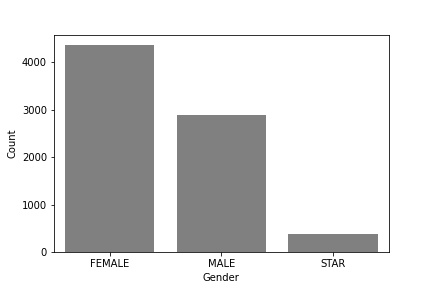
\includegraphics[width=\linewidth]{reports/figures/num_per_gender.jpg}
    \caption{Bar plot of the number of students per gender. There are almost the same number of students per gender.}
    \label{fig:gender}
\end{figure}

\begin{figure}[h]
    \centering
    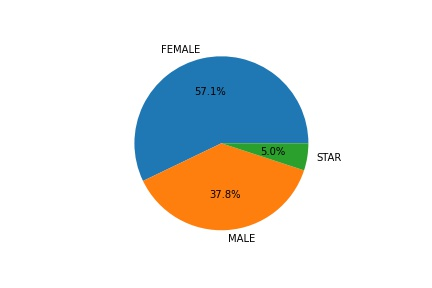
\includegraphics[width=\linewidth]{reports/figures/pie_chart.jpg}
    \caption{Proportion of students within each gener. STAR is an option reflecting if a student chooses to identify as neither male nor female.}
    \label{fig:pie_chart}
\end{figure}

Furthermore, we decide not to disclose based on the gender on the users since the difference between the percentage of females and males is not sufficiently large as shown in Figures \ref{fig:gender} and \ref{fig:pie_chart}. Finally, we found that the vast majority of students on the platform belong to year groups Gymnasium - 1. Jahr ($0.24 \%$ of the users) and Gymnasium - 2. Jahr ($0.16 \%$ of the users), the first group being the largest.

\section{Data Processing} \label{data:cleaning}

%{\color{red}
%\begin{itemize}
%    \item (MARIA) Data cleaning approaches: what is removed and rationale; changes in shape of dataset.
%\end{itemize}
%}

In the data processing phase, we first remove users with no transaction data (i.e. we keep users that are both in the events table and in the transactions table). To continue, inactive users will also be removed from our dataset since we consider that they are not using the platform enough to extract any valuable conclusion from them.

\begin{table*}[h]
  \caption{Features obtained after the cleaning process.}
  \label{tab:features}
  \begin{tabular}{cl}
    \toprule
    \textbf{Feature}&\textbf{Description}\\
    \midrule
    $\texttt{user\_id}$ & identifier of the user of the educational platform \\
    $\texttt{timestamp}$ & timestamp information of when the action was performed \\
    $\texttt{week}$ & derived from the feature $\texttt{timestamp}$, it corresponds to the week when the action was performed \\
    $\texttt{category}$ & classification of the action performed \\
    $\texttt{action}$ & type of action performed \\
    $\texttt{start\_time}$ & start time of the action \\
    $\texttt{commit\_time}$ & commit time of the action \\
    $\texttt{num\_checks}$ & total number of level checks that the user with $\texttt{user\_id}$ has performed \\
    $\texttt{nun\_participations}$ & total number of $\texttt{SUBMIT\_ANSWER}$ and $\texttt{GO\_TO\_THEORY}$ actions performed by an user of the platform \\
    $\texttt{num\_actions\_per\_week}$ & total number of significant actions performed by a particular user in a particular week \\
    $\texttt{num\_weeks\_per\_user}$ & total number of significant weeks performed by a particular user \\
    \bottomrule
    \end{tabular}
\end{table*}

Inactive students are students that are in one of the following situations:
\begin{itemize}
\item Students that have never performed a level check.
\item Students that have not performed any $\texttt{GO\_TO\_THEORY}$ action and neither any $\texttt{SUBMIT\_ANSWER}$ action.
\item Students that have at least two significant weeks. A \emph{significant week} is defined as a week with at least five significant actions. Moreover, the \emph{significant actions} are the actions in the event table that are linked through the transaction token to the transactions table. As a consequence, we will exclude actions like $\texttt{LOGIN}$, $\texttt{LOGOUT}$ or $\texttt{NAVIGATE\_DASHBOARD}$ from the list of significant actions.
\end{itemize}
Since our goal is to predict users' success in level checks based on their regularity in time, we are not interested in users who did not perform any level check. Moreover, we will remove untrackable students: those who never did any training question or theory reading event. The justification of the cleaning decision is simply that we are not interested in users that have not performed any training or preparation for the level checks because we cannot measure their regularity (since they have not used the platform enough).

Finally, we will remove users that have not been using the educational platform sufficiently during several weeks. Thus, we remove users with less than two significant weeks since we want to have data from different weeks to apply time series techniques. In addition, a significant week is defined like above since we consider that a student can reach the minimum of five significant actions per week in the platform very easily.

Additionally, features that are not useful for our study have been removed. The removed features are the following: $\texttt{transaction\_id}$, $\texttt{transaction\_token}$, $\texttt{document\_id}$, $\texttt{document\_version}$, $\texttt{user\_agent}$, $\texttt{validation}$, $\texttt{solution}$, \\ $\texttt{type}$, $\texttt{learn\_session\_id}$, $\texttt{topic\_id}$, $\texttt{is\_closed}$, $\texttt{type\_id}$, \\ $\texttt{is\_accepted}$, $\texttt{event\_id}$, $\texttt{session\_id}$, $\texttt{tracking\_data}$, \\ $\texttt{event\_type}$. Also, we are dropping the $\texttt{evaluation}$ and $\texttt{input}$ columns because we are not interested in whether a question is correct or not but in the result obtained in the whole level check.

Moreover, the timestamp we get from the original raw data will be transformed to a $\texttt{datetime}$ object via the function $\texttt{to\_datetime}$ of the pandas library taking into account the fact that the timestamp given is in milliseconds to further extract the week number. We need to compute the week number to extract features such as the $\texttt{num\_actions\_per\_week}$ or $\texttt{num\_weeks\_per\_user}$ because we want to analyse the behaviour of the students over time.

%Time series will be used to check if regular students will perform better than those who do not have regular habits when using the platform. In other words, does regularity influence a student’s performance in the level checks done on the platform?

Our dataset after the cleaning process consists of $790,425$ rows corresponding to actions of users on the platform. For each row, the features shown in Table \ref{tab:features} are listed as columns.

The information corresponding to the level checks performed by the users of the educational platform is located in the $\texttt{learn\_sessions\_transactions}$ table and can be linked to the $\texttt{transactions}$ table via the $\texttt{transaction\_id}$. After fetching all the level checks' dates, we create our labels to represent a measure of the learning. Indeed, we track changes in the mastery score for each level check and attribute a label of $1$ for the level checks featuring a mastery score improvement, and a label of $0$ for the ones featuring a decreasing mastery score. Then, as the chosen granularity is \textit{weekly}, we must aggregate all the level checks happening the same week for the same or different topics. To do so, we choose a simple approach by attributing to the given week the \textit{majority label} i.e. the level check week gets attributed the label of the majority of the level checks occurring during the week.

Therefore, each \textbf{sample} in our classification training data is constituted of chosen \textbf{features} and a \textbf{label}. The features (varying depending on the selected approach) are information up to a specific week preceeding the level check week. The label is the result of the aggregated change in mastery score i.e. whether the student mostly improved its level check score or decreased it. See section \ref{sec:propapp} for the details on each approach to illustrate the features-label in each case.

\begin{figure}
     \centering
     \begin{subfigure}[b]{\linewidth}
         \centering
         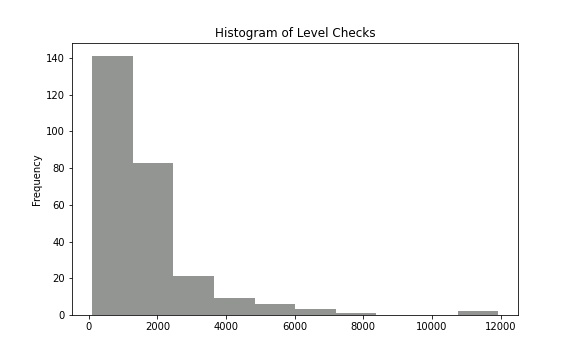
\includegraphics[width=0.82\linewidth]{reports/figures/histogram_level_checks.jpg}
         \caption{Histogram of the number of \emph{level checks} performed by the users of the platform.}
         \label{fig:level_cheks}
     \end{subfigure}
     \hfill
     \begin{subfigure}[b]{\linewidth}
         \centering
         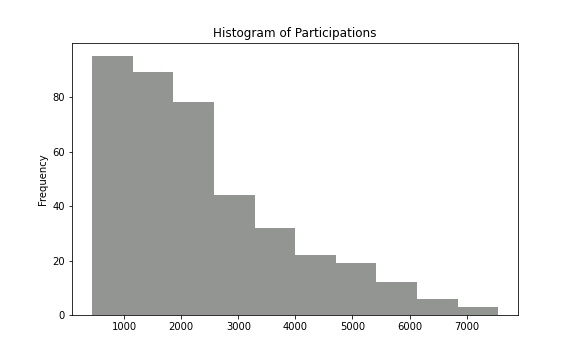
\includegraphics[width=0.82\linewidth]{reports/figures/histogram_num_participations.jpg}
         \caption{Histogram of the number of \emph{participations} performed by the users of the platform.}
         \label{fig:participations}
     \end{subfigure}
     \medskip
     \begin{subfigure}[b]{\linewidth}
         \centering
         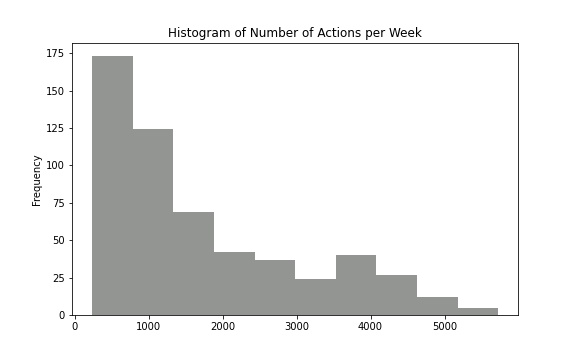
\includegraphics[width=0.82\linewidth]{reports/figures/histogram_number_of_actions_per_week.jpg}
         \caption{Histogram of the number of \emph{actions per week} performed by the users of the platform.}
         \label{fig:actions_per_week}
     \end{subfigure}
     \hfill
     \begin{subfigure}[b]{\linewidth}
         \centering
         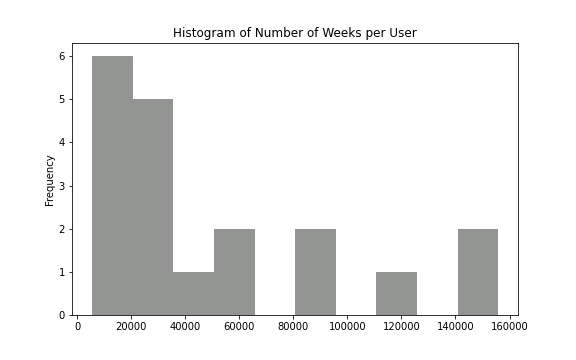
\includegraphics[width=0.82\linewidth]{reports/figures/histogram_number_of_weeks_per_user.jpg}
         \caption{Histogram of the number of \emph{weeks per user} in the platform.}
         \label{fig:weeks_per_user}
     \end{subfigure}
        \caption{Histograms of some of the numerical features presented.}
        \label{fig:histograms}
\end{figure}

By plotting the histograms of some of the numerical features, see Figure \ref{fig:histograms} for examples, it is clear that counting student \textit{actions} results in a positively skewed distribution, which demonstrates that few students have very high action counts on the platform.

\section{The Proposed Approaches}\label{sec:propapp}

We proceed onto experiments separated in 2 different approaches. Each of these approaches features a \textbf{clustering} and a \textbf{classification} part. Both techniques are applied to a different set of features to avoid data leakage through the experiment. They are chosen for the following reasons:

\begin{itemize}
    \item \textbf{Clustering} - The goal is to try to \textbf{identify and separate} according to behaviors detected in the raw data. This is a first naive approach towards grouping students with similar learning processes. Moreover, in an attempt to leverage the clustering, we also train a classifier for each clustered group. We hope to increase the classifier's accuracy by proceeding this way.
    \item \textbf{Classification} - This technique is used to separate classes according to our created labels. Therefore, we train a group of classifiers on a class-balanced training set. The group of classifiers includes 1 classifier for the whole training data, and 1 classifier per cluster. Its aim is to measure the predictive potential of the data regarding students' improvement. %Then, if the classification technique allows it, we retrieve and analyze the classifier's coefficients to gain insights on the features important for the classification.
\end{itemize}

See Figure \ref{fig:teaser} for a flowchart depiction of our methodology. 

\subsection{A1}\label{subsec:A1}
%{\color{red} (NICO) Description of methodology.}

The first approach features a \textit{time-agnostic} (no time dimension in the data) clustering and a time series classification. We describe both.

The \textbf{clustering} is performed based on a set of time agnostic features for each user. The features are computed over the whole study period of 40 weeks. They include: \textbf{counts of each significant action} (an action with a transaction token); \textbf{length of time spent} on the platform, and a set of so-called \textbf{regularity features} \cite{quantifyreg}. The latter is a set of metrics which measure to what extent user patterns repeat of chosen time periods, for example over hours of the day, days of the week, or weeks of the month. For instance, one feature, \texttt{PWD} -- an abbreviation of \textit{peak on weekday} -- measures if a users activity is concentrated around days of the week, based on the entropy of the histogram of the user's weekly activity. Figure \ref{fig:PWHex} illustrates the counts that the \texttt{PWD} metric is measuring. We refer the reader to \cite{quantifyreg} to find a detailed description of all of the features. Moreover, we use the \textbf{K-Means clustering} technique together with the \textbf{Silhouette Score} measure in order to compute the optimal number of cluster. K-Means is selected as it is a simple and scalable algorithm which produced reasonable computation times and results.

The \textbf{classification} is done over a set of time series. Contrary to the clustering phase during which each user in the training set corresponds to a sample, the classification uses time series, one for each level check. The training sample is formed by the weekly data for the student having the level check, up to the week preceding the level check. The weekly data includes the total \textit{number of actions per week}, the \textbf{time spent} on the platform during this week, \textbf{count of actions} for the selected relevant actions. Please see Figure \ref{tab:A1_feature_vectors} for a complete list of the feature aliases. Moreover, we use the \emph{tslearn} \cite{tslearn} library providing us with a collection of machine learning techniques adapted to time series. Among the proposed classicators, we select a \textbf{time series support vector} and a \textbf{time series K-NN} classification technique. Further details on their use are provided in section \ref{sec:results}.

\begin{table}[h]
    \centering
    \caption{Features details for clustering and classification in approach 1. For details regarding the regularity metrics, please refer to section \ref{subsec:A1} and \cite{quantifyreg}.}
    \begin{tabular}{|c|c|}
    \hline
        Clustering Features & Classification Features \\ \hline
        \texttt{PHD} & \texttt{num\_actions\_per\_week} \\ 
        \texttt{PWD} & \texttt{elapsed\_time} \\
        \texttt{WS1} & \texttt{REVIEW\_TASK} \\ 
        \texttt{WS2} &\texttt{SKIP} \\ 
        \texttt{WS3} &\texttt{CLOSE} \\ 
        \texttt{FDH} &\texttt{SUBMIT\_ANSWER} \\ 
        \texttt{FWH} &\texttt{GO\_TO\_THEORY} \\ 
        \texttt{FWD} &\texttt{NEXT} \\ 
        &\texttt{VIEW\_QUESTION} \\ 
        &\texttt{GO\_TO\_BUG\_REPORT} \\ 
        &\texttt{OPEN\_FEEDBACK} \\ 
        &\texttt{CLOSE\_FEEDBACK} \\ 
        &\texttt{GO\_TO\_COMMENTS} \\ 
        &\texttt{SHARE} \\ 
        &\texttt{REQUEST\_HINT} \\ \hline
    \end{tabular}
    \label{tab:A1_feature_vectors}
\end{table}

\begin{figure}
    \centering
    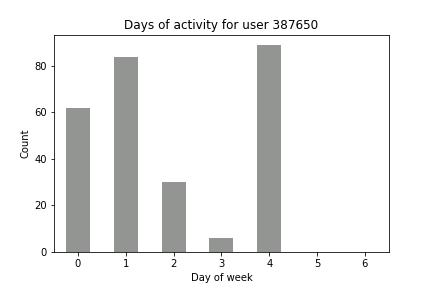
\includegraphics[width=\linewidth]{reports/figures/PWHex.jpg}
    \caption{Illustrative plot of daily activity for user 387650. We find that this user completes significant actions on every day of the week except for the weekend, with peaks on Tuesday and Friday.}
    \label{fig:PWHex}
\end{figure}


\subsection{A2}\label{subsec:A2}
%{\color{red}(NICO + MARIA) Description of methodology.}     

The second approach inverts the type of features fed to the clustering and classification. In this approach, we first cluster our user time series, and then feed time agnostic features to the classifier. We describe both.

The \textbf{clustering} is done on the time series of the users. Similarly to the time series classification of approach 1, we aggregate data on a weekly basis. Thus for each user, we create a vector per week containing the following information: total \textbf{number of actions} performed during the week, \textbf{time spent} on the platform during the week, and the \textbf{count of some selected relevant actions} for the week. Please see table \ref{tab:A2_feature_vectors} for a complete list of the features aliases. Moreover, we again use the methods from the  \emph{tslearn} \cite{tslearn} library. Here we use a \textbf{time series K-Means} clustering technique and a \textbf{kernelized version of the time series K-Means} i.e. a kernel function is applied to the time series before performing K-Means.

\begin{table}[h]
    \centering
    \caption{Features details for clustering and classification in approach 2.}
    \begin{tabular}{|c|c|}
    \hline
        Clustering Features & Classification Features \\ \hline
        \texttt{num\_actions\_per\_week} & \texttt{num\_weeks\_on}\\ 
        \texttt{elapsed\_time} & \texttt{num\_actions\_per\_week}\footnote{Time agnostic feature. Different from the time series' weekly feature.}\\
        \texttt{REVIEW\_TASK} & \texttt{FDH}\\ 
        \texttt{SKIP} & \texttt{FWH} \\ 
        \texttt{CLOSE} & \texttt{FWD} \\ 
        \texttt{SUBMIT\_ANSWER} & \texttt{eng\_score}\\ 
        \texttt{GO\_TO\_THEORY} & \\ 
        \texttt{NEXT} & \\ 
        \texttt{VIEW\_QUESTION} & \\ 
        \texttt{GO\_TO\_BUG\_REPORT} & \\ 
        \texttt{OPEN\_FEEDBACK} & \\ 
        \texttt{CLOSE\_FEEDBACK} & \\ 
        \texttt{GO\_TO\_COMMENTS} & \\ 
        \texttt{SHARE} & \\ 
        \texttt{REQUEST\_HINT} & \\ \hline
    \end{tabular}
    \label{tab:A2_feature_vectors}
\end{table}


\begin{table*}[!ht]
  \caption{Description of the time agnostic, aggregated features used in approach 2 for a given user $i$ for all data recorded on the platform before level check $t$.}
  \label{tab:A2features}
  \begin{tabular}{cl}
    \toprule
    \textbf{Feature}&\textbf{Description}\\
    \midrule
    $\texttt{num\_weeks\_on}$ & number of weeks recorded having used the platform\\
    $\texttt{num\_actions\_per\_week}$\footnote{Time agnostic feature. Different from the time series' weekly feature.} & average number of actions with a transaction token per week\\
    $\texttt{FDH}$ & measures the extent to which the hourly pattern of user’s activities is repeating over days \\
    $\texttt{FWH}$ & measures if the hourly pattern of activities is repeating over weeks\\
    $\texttt{FWD}$ & captures if the daily pattern of activities is repeating over weeks\\
    $\texttt{eng\_score}$ & binary indicator of `high' user engagement\\
    \bottomrule
    \end{tabular}
\end{table*}

\begin{figure}
    \centering
    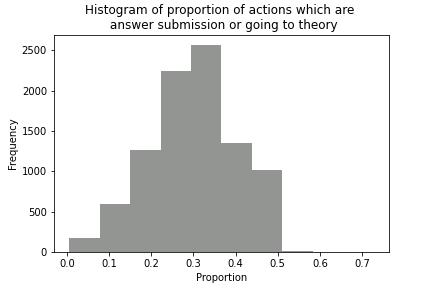
\includegraphics[width=\linewidth]{reports/figures/eng_score_hist.jpg}
    \caption{Proportion of actions which are answer submissions or going to theory.}
    \label{fig:eng_score}
\end{figure}


\begin{figure}
    \centering
    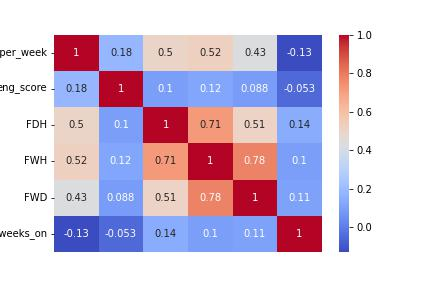
\includegraphics[width=\linewidth]{reports/figures/feature_corr.jpg}
    \caption{Correlation heatmap between all the features. Note we have relabelled $\texttt{num\_actions\_per\_week}$ to \#actions and $\texttt{num\_weeks\_on}$ to \#weeks for display purposes.}
    \label{fig:feature_corr}
\end{figure}


%{\color{red}Clustering...}

For the \textbf{classification}, a \textbf{decision tree classifier} and a \textbf{random forest classifier} based on behavioural features were chosen due to the very interpretable nature of such models. Indeed, it allows for the categorisation of students based on quantitative metrics on usage of the platform, while also ranking the importance of the behavioural features, which helps us in answering our research question. 

Let $N$ be the number of users and $L_i$ be the number of level checks user $i$ has completed. For each $i \in \{1,\ldots,N\}$ and $t \in \{1, \ldots, L_i\}$, the data fed into the decision tree classifier is a vector $x_i^t = (x_{i1}^t, x_{i2}^t, \ldots, x_{i6}^t)$, where $x_{i1}$ is a positive integer, $x_{ik}$ for $k=2,3,4$ is a positive real number and $x_{i6} \in \{0,1\}$. The features $x_{ik}$ for $k=1,\ldots, 6$ are listed in Table 
\ref{tab:A2features}. Note the index $t$ is ordered in time. 

To elaborate further, $x_{ik}$ for $k=2,3,4$ are \textbf{frequency-based} regularity features taken from \cite{quantifyreg}. In brief, these features find the spectral density of the time series generated by recording student actions, and subsequently detecting any important frequencies within the time series. This serves to identify with what frequency students repeat certain patterns of specified time periods: for the features \texttt{FDH}, \texttt{FWH} and \texttt{FWD} these are hours-across-day patterns (e.g. a user is active at 8AM every morning), hour-across-week patterns (e.g. a user is active 8AM every \textit{Monday}) and days-across-week (e.g. a user is active every \textit{Monday}) patterns respectively. Notably, the features decrease in granularity, while each capturing interesting snapshots of student behaviour. 

An `engagement score', inspired by \cite{student_engagement}, records whether a student demonstrated that they performed activities directly related to learning (submitting answers to questions and going to theory sections of the app) more than other students. To quantify this, if for a given user, the two aforementioned actions comprised more than $25\%$ of all actions recorded in $\texttt{num\_actions\_per\_week}$, then they were given an engagement score of $1$ and $0$ otherwise. We remark that each of these features aim to quantify some form of consistent behavioural pattern on the platform, ranging from simply being present on the platform, to using it in a repeated manner over a long period of time. 

\section{Experiments and Results}\label{sec:results}

For each of the aforementioned approaches, we derive a series of experiments. In this section we detail the design of the experiments and then explore the results.
%{\color{red}NICO (A1), MARIA (A2)}
\subsection{Experiments}
\subsubsection{A1}
For the first approach, the clustering was done using the \textbf{K-Means} algorithm. For this experiment, we finetune the number of clusters \texttt{k} $\in \{2,3,\ldots, 10\}$. Then we use the \textbf{Silhouette Score} in order to see which clustering is most coherent to our data. %\textit{Let us recall that the silhouette score evaluates how well distinguishable and identified the clusters are by rating their centers’ individuality and preciseness. It ranges from $1$ (perfectly differentiable and identified clusters) to $-1$ (overlapping clusters with close centers).}

The classification is done using 2 different classification techniques applied to time series. Namely, we classify for the clustered and non-clustered setting using the \texttt{TimeSeriesSVC} (support-vector technique) and \\ \texttt{KNeighborsTimeSeriesClassifier} (K-NN classification technique). For the former method, we could not perform experiments by varying the \texttt{kernel} parameter as the \textit{Global Alignment Kernel} \texttt{gak} \textbf{kernel} is the only one working for the time series classification. \textit{The GAK kernel is responsible for aligning the different time series before classification}. For the latter method, we had the possibility to tune the \textbf{number of considered neighbors}. However preliminary results with the default parameter showed that the model performed significantly worse than its support-vector counterpart. Therefore, we did not perform experiments on this dimension of the model. The default parameter used was \texttt{k=3}. Finally due to the significant amount of time necessary to train the classifier, we chose to perform experiments by varying the \textbf{number of samples} used for training in the range $[10, 3953]$. Let us note that the upper bound of this range is not reached for all experiments, however all experiments go up to at least $828$ samples.

\subsubsection{A2}
For the second approach, the clustering was done using 2 different time series clustering techniques. The techniques are \texttt{TimeSeriesKMeans} (K-NN based clustering techniques) and \texttt{KernelKMean} (variation of the former applying a kernel function before clustering). For the first technique, we vary the \textbf{number of clusters} in the integer range $[2, 6]$, the \textbf{maximum iterations} performed by the algorithm in the list $[50, 100]$, the tolerance criterion to indicate convergence in the list $[1e-5, 1e-6, 1e-7]$, the \textbf{distance metric} in the list $[\texttt{euclidean}, \texttt{dtw}]$, and whether the algorithm should use \textbf{inertia} or not. the second technique features hyper-parameter tuning on the applied kernel function in the list $[\texttt{gak}, \texttt{linear}, \texttt{poly}, \texttt{sigmoid}]$, and the number of clusters in the integer range $[2, 4]$.

In the second part, we performed two experiments. In the first experiment, the classification step is carried out with all the behavioral features shown in Table \ref{tab:A2features}, whereas in the second experiment we left out the feature $\texttt{num\_weeks\_on}$.

Both a \textbf{Decision Tree Classifier} and a \textbf{Random Forest Classifier} were trained on both experiments using the whole dataset since the clustering was not relevant. Hyperparameter tunning was performed using \textbf{Randomized Search} to determine the best parameters of each of the models using the grids described in Tables \ref{tab:grid_dt} and \ref{tab:grid_rf}.

The parameters tuned for each of the models in both of the experiments with their respective best combinations can be found in the Tables \ref{tab:dc_1}, \ref{tab:dc_2}, \ref{tab:rf_1} and \ref{tab:rf_2}.

The Figures \ref{fig:hyp_decision_1} and \ref{fig:hyp_decision_2} show accuracy results for several trainings done with different combinations of the parameters of the Decision Tree Classifier for the first and the second experiment respectively. Equivalently, the Figures \ref{fig:hyp_forest_1} and \ref{fig:hyp_forest_2} show accuracy results for several trainings done with different combinations of the parameters of the Random Forest Classifier for the first and the second experiment respectively.

The feature importance of each of the classifiers in both experiments is shown in Figures \ref{fig:fi_dc_1},
\ref{fig:fi_dc_2}, \ref{fig:fi_rf_1} and \ref{fig:fi_rf_2}. As we can see, the most important feature in Experiment 1 is $\texttt{num\_weeks\_on}$ whereas in Experiment 2 is $\texttt{num\_actions\_per\_week}$. Surpringsingly, the regularity features computed ($\texttt{FDH}$, $\texttt{FWH}$, $\texttt{FWD}$ and $\texttt{eng\_score}$) have a low importance.

\subsection{Model Results and Evaluation}\label{subsec:eval_results}

After having run the experiments, we measure the results using different metrics. These metrics depend on the clustering or classification step in the approach. For the clustering step, we use the \textbf{Silhouette Score} to measure the cluster relation to our data. For the classification step, we use 6 different metrics \cite{scikit-learn}, namely the \textbf{accuracy} (percentage of samples correctly classified), the \textbf{balanced accuracy} (accuracy taking class balance into account), the \textbf{adjusted balanced accuracy} (balanced accuracy accounting for chance in classification), the \textbf{F1 score} (harmonic mean of the precision and recall), the \textbf{weighted F1 score} (F1 score weighted by class support) and \textbf{Matthew's coefficient} (binary classification correlation coefficient).

\subsubsection{A1}

The silhouette scores linked to the clustering results features a clear downward trend (see Figure \ref{fig:A1_clustering_silhouette}). Indeed, the maximum score of \textbf{0.66} is reached for \textbf{2} clusters. It then drops down to 0.53 at 3 clusters and keeps decreasing. The two groups feature \textbf{2'132} and \textbf{344} samples respectively, denoting an important size imbalance. Therefore, we ask ourselves if the clustering is relevant and proceed to the classification with both clustered and non-clustered experiments.

\begin{figure}[h]
    \centering
    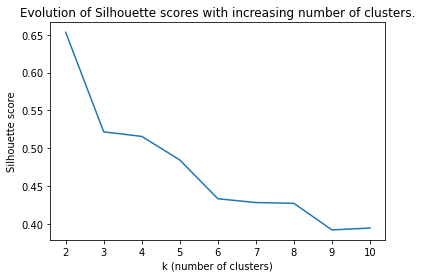
\includegraphics[width=0.4\textwidth]{reports/figures/A1_clustering_kmeans.png}
    \caption{Silhouette score evolution with the number of clusters in A1 (time agnostic clustering).}
    \label{fig:A1_clustering_silhouette}
\end{figure}

Let us start by comparing the classification methods in the global (no clustering) setup. For \texttt{TimeSeriesSVC}, we can see that all scores increase significantly up to \textbf{828} samples (see figure \ref{fig:A1_classification_svc_noscluter}). For the accuracy and F1-score, we reach a maximum of \textbf{79.9\%} accuracy for 828 samples (79.6\% for 1101 samples) and \textbf{86.8\%} F1-score for 1101 samples (86.6\% for 828 samples). Finally, we see a maximum correlation of \textbf{+0.469} (Matthew’s coefficient) at 828 samples.
However, using the \\ \texttt{KNeighboursTimeSeriesClassifier}, the accuracy seems to oscillate between \textbf{43\%} and \textbf{44.6\%}, and F1-score oscillates between \textbf{45.1\%} and \textbf{47.2\%} (see figure \ref{fig:A1_classification_knn_nocluster}). Both scores are below 50\% and no clear trend can be observed in any of the metrics. Finally the maximum correlation coefficient is \textbf{+0.088} which is obtained with 10 samples.

Then, by looking at the clustered experiments, we can further confirm some insights.
For \texttt{TimeSeriesSVC}, regardless of the clusters we observe that all scores increase sharply until \textbf{667} samples training-set-size (cluster 0) and \textbf{572} samples (cluster 1) (see figures \ref{fig:A1_classification_svc_cluster0} and \ref{fig:A1_classification_svc_cluster1}). Following this point, the scores seem to decrease slightly for cluster 0 and stay steady for cluster 1. This variation in cluster 0 could be interpreted as overfitting. However the highest accuracy and F1-score are confidently reached for \textbf{886} samples (accuracy: \textbf{79.9\%}; F1-score: \textbf{86.8\%}) for cluster 0 and \textbf{853} samples (accuracy: \textbf{75.6\%}; F1-score: \textbf{84.2\%}) for cluster 1. Confidence comes from the fact that cluster 0 evaluates classifiers trained up to 3’953 samples and cluster 1 up to 1’556 samples, both of which are significantly higher than the number of samples for which we observe the best scores.
For \\ \texttt{KNeighboursTimeSeriesClassifier}, the results are very different between cluster 0 and cluster 1. Let us note that cluster 0 evaluates results only \textbf{4} times up to 886 samples, whereas cluster 1 has \textbf{29} evaluations up to 994 samples. However the trends are still significantly different (see figures \ref{fig:A1_classification_knn_cluster0} and \ref{fig:A1_classification_knn_cluster1}). 
In cluster 0, the best accuracy and F1-score are reached for \textbf{10} samples with \textbf{50.3\%} accuracy and \textbf{57.4\%} F1-score.
Cluster 1 has a more consistent behavior, and the best accuracy is reached at \textbf{115} samples with \textbf{61.7\%}. Best F1-score is also reached at \textbf{115} samples with \textbf{73.2\%}. Moreover, adjusted accuracy and correlation oscillate around \textbf{0} with best scores of \textbf{8.3\%} and \textbf{0.099} at \textbf{10} samples. There is no trend for these two metrics as negative values are observed as early as \textbf{200} samples, before going back to positive values at around \textbf{400} samples and then negative again around \textbf{750} samples.

\begin{figure*}[h]
    \centering
    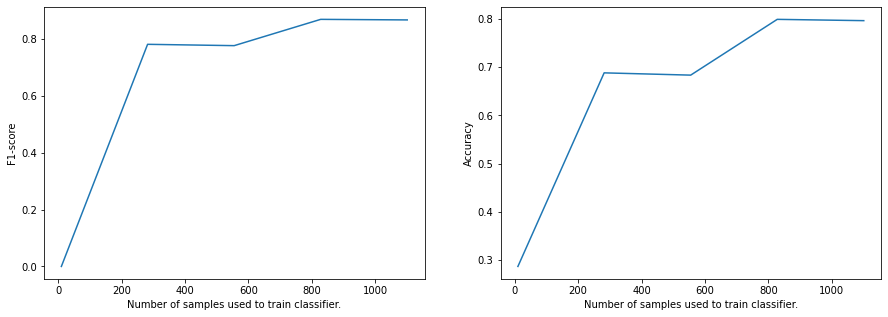
\includegraphics[width=\linewidth]{reports/figures/A1_classification_svc_nocluster.png}
    \caption{Evolution of F1-score and accuracy with the number of samples for the support vector classification in A1 (best performing in approach 1).}
    \label{fig:A1_classification_svc_noscluter}
\end{figure*}

\subsubsection{A2}

The clustering for the second approach featured mixed silhouette scores depending on the technique. Indeed, the time series KMeans \texttt{TimeSeriesKMeans} clustering reached its highest silhouette score of \textbf{0.987} for the following configuration: \textbf{2} clusters, \textbf{50} iterations max, tolerance of \textbf{1e-05}, \textbf{euclidian} metric, and with \textbf{inertia} (see figure \ref{fig:A2_clustering_german_kmeans}). However, the cluster imbalance is high with cluster 0 having only 2 samples.
On the other hand, the time series kernel (\texttt{KernelKMeans}) clustering performed poorly. The trend goes downward with the number of clusters starting from the beginning. The highest silhouette score is reached at \textbf{0.137} with the \textbf{sigmoid kernel} function and \textbf{2} clusters (see figure \ref{fig:A2_clustering_math_kernel}). The score goes below 0 as soon as the number of clusters gets higher than 2. Moreover there is no distinguishable difference between the performances of the different kernels.

The best results were obtained by the \textbf{Random Forest classifier} trained in \textbf{Experiment 1}. The values obtained for the different metrics described at the beginning of this section can be seen in Table \ref{tab:rf_1_table_results}, where we obtain \textbf{$97.8\%$ accuracy} and \textbf{$98.5\%$ F1-score} for $962$ samples. However, when we trained the \textbf{Random Forest Classifier} in \textbf{Experiment 2}, we obtain \textbf{$56.1\%$ accuracy} and \textbf{$65.8\%$ F1-score} (results shown in table \ref{tab:rf_2_table_results}). This significantly drop in the accuracy when we performed Experiment 2 may be due to a lack of expressiveness of the features used. The results obtain for the Decision Tree Classifiers trained on Experiments 1 and 2 can be found in Tables \ref{tab:dc_1_table_results} and \ref{tab:dc_2_table_results}.

\begin{table*}[h]
  \caption{\textbf{Accuracy}, \textbf{balanced accuracy}, \textbf{adjusted balanced accuracy}, \textbf{F1 score}, \textbf{weighted F1 score} and \textbf{Matthew's coefficient} for the \emph{Random Forest Classifier} trained in \emph{Experiment 1}.}
  \label{tab:rf_1_table_results}
  \begin{tabular}{cllllll}
    \toprule
    \textbf{Samples}&\textbf{Accuracy}&\textbf{Balanced Accuracy}&\textbf{Adj. Balanced Accuracy}&\textbf{F1}&\textbf{Weighted F1}&\textbf{Matthew's coeff.}\\
    \midrule
    $10$ & $0.888$ & $0.917$ & $0.834$ & $0.918$ & $0.893$ & $0.763$\\
    $168$ & $0.903$ & $0.930$ & $0.860$ & $0.930$ & $0.907$ & $0.792$\\
    $327$ & $0.913$ & $0.941$ & $0.881$ & $0.938$ & $0.917$ & $0.814$\\
    $486$ & $0.975$ & $0.981$ & $0.963$ & $0.983$ & $0.975$ & $0.939$\\
    $644$ & $0.978$ & $0.982$ & $0.963$ & $0.985$ & $0.978$ & $0.945$\\
    $803$ & $0.984$ & $0.985$ & $0.969$ & $0.989$ & $0.984$ & $0.960$\\
    $962$ & $0.987$ & $0.988$ & $0.976$ & $0.991$ & $0.987$ & $0.967$\\
    \bottomrule
    \end{tabular}
\end{table*}

Figures \ref{fig:results_rf_1} and \ref{fig:results_rf_2} plot the accuracy and the F1-score against the number of samples in both experiments for the Random Forest model. Analogous graphs are shown in Figures \ref{fig:results_dt_1} and \ref{fig:results_dt_2}.

 \begin{figure*}[h]
     \centering
     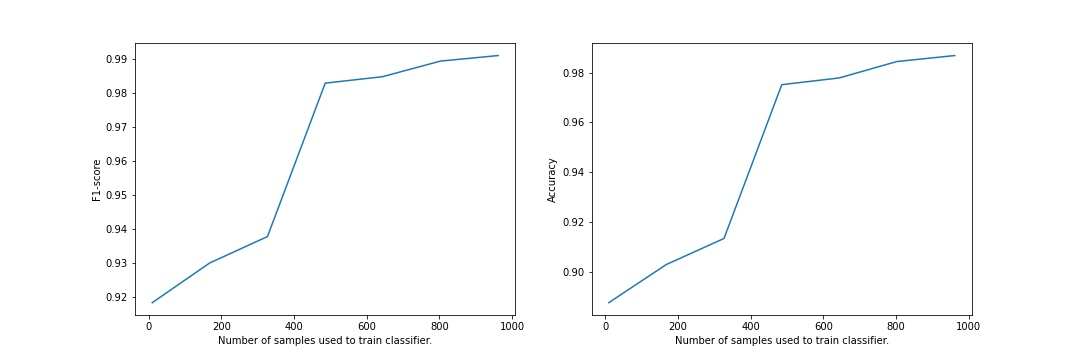
\includegraphics[width=\linewidth]{reports/figures/results_rf_1.jpg}
     \caption{\emph{Accuracy} and \emph{F1-score} against number of samples of the \emph{Random Forest Classifier} trained in \emph{Experiment 1}.}
     \label{fig:results_rf_1}
 \end{figure*}
 
  \begin{figure*}[h]
     \centering
     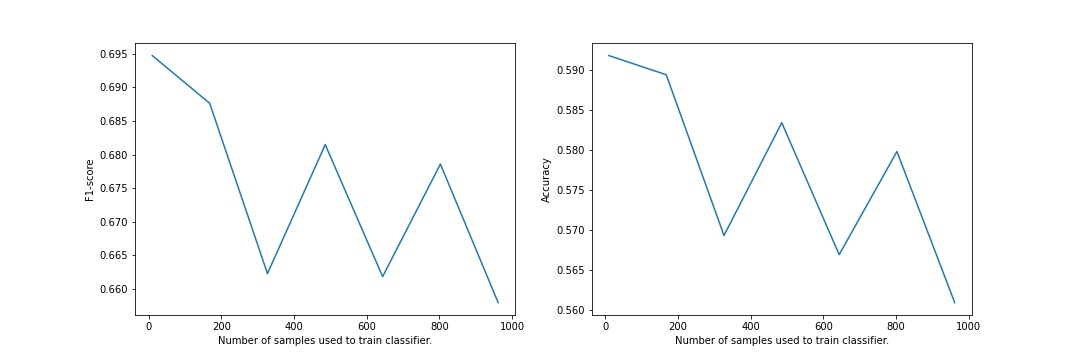
\includegraphics[width=\linewidth]{reports/figures/results_rf_2.jpg}
     \caption{\emph{Accuracy} and \emph{F1-score} against number of samples of the \emph{Random Forest Classifier} trained in \emph{Experiment 2}.}
     \label{fig:results_rf_2}
 \end{figure*}

\section{Discussion}\label{sec:discussion}

%{\color{red}
%\begin{itemize}
%\item Justification: (NICO) Choice to switch the order of clustering and classification going from A1 to A2. 
%    \item Justification: (NICO + MARIA) Failure of clustering
%    \item Justification: (NICO +MARIA) Wild variation in accuracy upon changing elements of the modelling procedure/features
%\end{itemize}

%}
Let us first further elaborate on the relevance of our two approaches. Moving from A1 to A2 we switched the order of the clustering and classification steps, in which our use of time series data was an attempt at verifying which type of data was best suited for each specific type of classification. Moreover splitting the approaches in 2 steps allows us to use 2 different kinds of data in the same experiment and avoid data leakage as the features are completely different.

Another observation is that in both experiments, clustering did not bring much information or precision to the classification step. Indeed, even after hyperparameter fine-tuning, the time series clustering produced an intractable clustering with one cluster having 2 samples only whereas the second cluster holds all the other users. We deduce from it that distance (even with kernel transformations) is not a representative metric to interpret an optimal learning behavior. With respect to the classification results, we conclude that the separation in various dimensions is a more adapted way to catch the underlying patterns in the data.

A remaining interrogation concerns the very volatile classification accuracy in the second approach. We suspect that there is an error in the data that we used, leading to some form of data leakage between the training and the evaluation. This could indeed explain the very high classification accuracy (97.8\%) and then the sudden drop following a feature removal. However, we were unable to find the mistake and can thus only formally state our doubts.

Our results demonstrate that differing patterns of student behaviours certainly influence their performance on the platform. We could not identify a specific optimal behavior, and our highest prediction accuracy confirmed the `common sense' answer to our question: the more time you spend on the platform, the better you will tend to achieve. Succinctly, consistency begets attainment. 

These results, however, highlight one key difficulty with our approach. Extracting a meaningful measure of human behaviour through myriad, anonymous clickstreams is a monumental task with many concerns and limitations \cite{meaningfulmeasures}. Human behaviour is an extremely nuanced piece of our being, and the advent of Big Data gives scientists a new avenue through which to understand it. Nevertheless, more advanced techniques and methods need to be developed in order to extract precise patterns that could reasonably have a causal effect on the outcome, as this is the ultimate goal; that is, for each student to have a personalised education. 





\section{Conclusion and Future Works}\label{sec:conclusion}

%{\color{red} To conclude ... summarise work}.
To conclude, this report details how we looked into student's behavior to improve the examinations results. It details the dataset and the processing work done to select features and samples to be used in our proposed approaches. Two approaches are then detailed to attempt to answer the research question. The first one features a clustering followed by a time series classification, whereas the second one starts with a time series clustering and follows with a time agnostic classification. Within each approach, we run various experiments, in order to fine tune our results and select the best models and methods. Very interestingly, we get promising results for our first approach with the best accuracy going up to 79.9\% with a non-clustered support vector classification over the designated set of features. More suprisingly, we reach a 97.8\% accuracy for the second approach, leading us to investigate our work. 

Put altogether, this project helped us assess the potential of machine learning methods to leverage real-life data and gain insights from production data. We built a full data processing pipeline and could try different methods to explore, process, transform and learn from it. The discussions in section \ref{sec:discussion} elaborate on our thoughts regarding the employed methods, their constraints and their limitations. However, we believe that our work paves the way for further in-depth research into Lernnavi's data and online learning platform insights in general. 

In future work, we suggest that the results of our work be used to inform an experiment in which the inverse approach is taken. That is, informed by data and neuroscientific and psychological literature, conduct a (conditionally) randomised experiment in which students are exposed to -- or, forced to exhibit -- a particular behaviour or structure, and appeal to the field of causal inference in order to determine any effect on attainment, by comparing and contrasting enforced behavioural patterns. For example, students might be use the platform solely as a homework device, or it might be used in conjunction with classroom learning. In this way, educators can begin to narrow the scope on what behavioural patterns lead to success, which could work in tandem with the development of machine learning models, in order to refine the patterns for which they search. 



%%
%% The acknowledgments section is defined using the "acks" environment
%% (and NOT an unnumbered section). This ensures the proper
%% identification of the section in the article metadata, and the
%% consistent spelling of the heading.
\begin{acks}
To Paola, for the sustained interest and really fruitful and engaging topical discussions.
\end{acks}

%%
%% The next two lines define the bibliography style to be used, and
%% the bibliography file.
\bibliographystyle{ACM-Reference-Format}
\bibliography{reports/refs.bib}


%%
%% If your work has an appendix, this is the place to put it.

\np 
\appendix
\onecolumn
\section{Appendix}
\subsection{Further Tables and Figures}

\begin{table*}[h]
  \caption{Feature description of the $\texttt{learn\_sessions\_transactions}$ dataset.}
  \label{tab:learn}
  \begin{tabular}{cl}
    \toprule
    \textbf{Feature}&\textbf{Description}\\
    \midrule
    $\texttt{learn\_session\_id}$ & unique identifier for each learn session \\
    $\texttt{transaction\_id}$ & transaction identifier, used to link with transactions table \\
    $\texttt{topicId}$ & identifier of the topic this session was about \\
    $\texttt{max\_num\_tasks}$ & maximum number of tasks included in this session (only relevant for the learn session) \\
    $\texttt{is\_closed}$ & if this session has been finished ($1$: finished; $0$: not finished) \\
    $\texttt{type\_id}$ & if this session is a learn or level check ($1$: learn; $2$: level check) \\
    $\texttt{is\_accepted}$ & if the user finally accepted the result of this session ($1$: accpeted; $0$: refused). \\
    \bottomrule
    \end{tabular}
\end{table*}

\begin{table*}[h]
  \caption{Feature description of the $\texttt{users}$ dataset.}
  \label{tab:users}
  \begin{tabular}{cl}
    \toprule
    \textbf{Feature}&\textbf{Description}\\
    \midrule
    $\texttt{user\_id}$ & personal identifier of user in database \\
    $\texttt{gender}$ & only three values: male, female or missing \\
    $\texttt{canton}$ & swiss canton \\
    $\texttt{class\_level}$ & school year in swiss system \\
    $\texttt{class\_code}$ & identifier of student's class. There are students that are using the platform as part of their school work \\
    \bottomrule
    \end{tabular}
\end{table*}

\begin{table*}[h]
  \caption{Feature description of the $\texttt{events}$ dataset.}
  \label{tab:events}
  \begin{tabular}{cl}
    \toprule
    \textbf{Feature}&\textbf{Description}\\
    \midrule
    $\texttt{event\_id}$ & identifier of event in database \\
    $\texttt{user\_id}$ & user who performed the event \\
    $\texttt{timestamp}$ & timestamp of event \\
    $\texttt{category}$ & classification of action (task, general, statistics, etc) \\
    $\texttt{action}$ & type of action performed \\
    $\texttt{event\_type}$ & whether the event required students to view or to click \\
    $\texttt{transaction\_token}$ & used to link to $\texttt{transactions}$ table \\
    $\texttt{session\_id}$ & during which session the event took place \\
    $\texttt{tracking\_data}$ & optional content associated to this event (e.g., the new points mastered for a topic) \\
    \bottomrule
    \end{tabular}
\end{table*}


\begin{table*}[h]
  \caption{Feature description of the $\texttt{transactions}$ dataset. The features $\texttt{document\_id}$ and $\texttt{document\_version}$ can be used to merge with the $\texttt{document}$ table}
  \label{tab:transactions}
  \begin{tabular}{cl}
    \toprule
    \textbf{Feature}&\textbf{Description}\\
    \midrule
    $\texttt{transaction\_id}$ & unique identifier for each transaction \\
    $\texttt{transaction\_token}$ & used to join with events table \\
    $\texttt{user\_id}$ & user who performed the transaction \\
    $\texttt{document\_id}$ & document that was answered in transaction \\
    $\texttt{document\_version}$ & version of document that was answered \\
    $\texttt{evaluation}$ & whether the user answered correctly or not. It is possible that it was only partially right \\
    $\texttt{input}$ & answer the user gave \\
    $\texttt{start\_time}$ & timestamp of when the user started answering \\
    $\texttt{commit\_time}$ & timestamp of when the user submitted the answer \\
    $\texttt{user\_agent}$ & the browser that the user used \\
    $\texttt{validation}$ & used to validate the format of the input \\
    $\texttt{solution}$ & solution to question \\
    $\texttt{type}$ & type of question \\
    \bottomrule
    \end{tabular}
\end{table*}

\begin{table*}[h]
  \caption{Table of metrics for the non-clustered support vector classification in approach 1.}
  \label{tab:A1_classification_svc_nocluster}
  \begin{tabular}{cllllll}
    \toprule
    Number of samples & accuracy & balancedaccuracy & adjusted balanced accuracy & f1 & f1 weighted & matthews\\
    \midrule
       10 & 0.287 & 0.500 & 0.000 & 0.000 & 0.128 & 0.000\\
      282 & 0.688 & 0.621 & 0.242 & 0.781 & 0.689 & 0.241\\
      555 & 0.683 & 0.620 & 0.240 & 0.776 & 0.685 & 0.237\\
      828 & 0.799 & 0.702 & 0.403 & 0.868 & 0.784 & 0.469\\
     1101 & 0.796 & 0.700 & 0.400 & 0.866 & 0.782 & 0.462\\
    \bottomrule
    \end{tabular}
\end{table*}

\begin{figure*}[h]
    \centering
    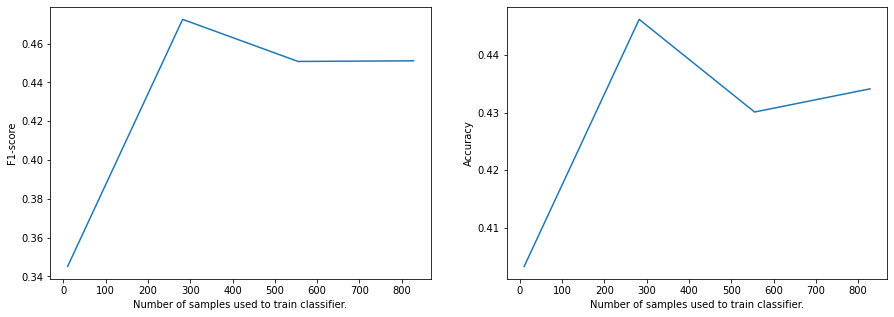
\includegraphics[width=\linewidth]{reports/figures/A1_classification_knn_nocluster.png}
    \caption{Evolution of F1 score and accuracy for the non-clustered KNN classification in approach 1.}
    \label{fig:A1_classification_knn_nocluster}
\end{figure*}

\begin{table*}[h]
  \caption{Table of metrics for the non-clustered KNN classification in approach 1.}
  \label{tab:A1_classification_knn_nocluster}
  \begin{tabular}{cllllll}
    \toprule
    Number of samples & accuracy & balancedaccuracy & adjusted balanced accuracy & f1 & f1 weighted & matthews\\
    \midrule
       10 & 0.403 & 0.539 & 0.078 & 0.345 & 0.376 & 0.088\\
      282 & 0.446 & 0.519 & 0.039 & 0.472 & 0.457 & 0.037\\
      555 & 0.430 & 0.506 & 0.012 & 0.451 & 0.438 & 0.011\\
      828 & 0.434 & 0.514 & 0.029 & 0.451 & 0.441 & 0.028\\
    \bottomrule
    \end{tabular}
\end{table*}

\begin{figure*}[h]
    \centering
    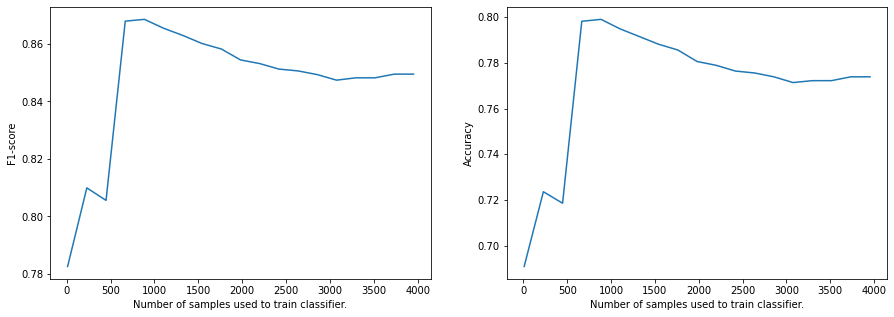
\includegraphics[width=\linewidth]{reports/figures/A1_classification_svc_cluster0.png}
    \caption{Evolution of F1 score and accuracy for the support vector classification in approach 1 (cluster 0).}
    \label{fig:A1_classification_svc_cluster0}
\end{figure*}

\begin{table*}[h]
  \caption{Table of metrics for the support vector classification in approach 1 (cluster 0).}
  \label{tab:A1_classification_svc_cluster0}
  \begin{tabular}{cllllll}
    \toprule
    Number of samples & accuracy & balancedaccuracy & adjusted balanced accuracy & f1 & f1 weighted & matthews\\
    \midrule
          10 & 0.691 & 0.627 & 0.254 & 0.783 & 0.694 & 0.249\\
      229 & 0.724 & 0.649 & 0.299 & 0.810 & 0.721 & 0.304\\
      448 & 0.719 & 0.647 & 0.294 & 0.806 & 0.717 & 0.297\\
      667 & 0.798 & 0.701 & 0.403 & 0.868 & 0.785 & 0.460\\
      886 & 0.799 & 0.702 & 0.404 & 0.869 & 0.786 & 0.462\\
     1105 & 0.795 & 0.699 & 0.398 & 0.865 & 0.782 & 0.452\\
     1324 & 0.791 & 0.697 & 0.393 & 0.863 & 0.779 & 0.444\\
     1543 & 0.788 & 0.696 & 0.392 & 0.860 & 0.777 & 0.437\\
     1762 & 0.786 & 0.694 & 0.389 & 0.858 & 0.775 & 0.431\\
     1981 & 0.781 & 0.691 & 0.382 & 0.854 & 0.770 & 0.420\\
     2200 & 0.779 & 0.690 & 0.379 & 0.853 & 0.769 & 0.416\\
     2419 & 0.776 & 0.688 & 0.376 & 0.851 & 0.767 & 0.410\\
     2638 & 0.776 & 0.687 & 0.375 & 0.851 & 0.766 & 0.409\\
     2857 & 0.774 & 0.686 & 0.372 & 0.849 & 0.765 & 0.405\\
     3076 & 0.771 & 0.684 & 0.369 & 0.847 & 0.762 & 0.399\\
     3295 & 0.772 & 0.684 & 0.368 & 0.848 & 0.763 & 0.400\\
     3514 & 0.772 & 0.684 & 0.368 & 0.848 & 0.763 & 0.400\\
     3734 & 0.774 & 0.685 & 0.371 & 0.849 & 0.764 & 0.404\\
     3953 & 0.774 & 0.685 & 0.371 & 0.849 & 0.764 & 0.404\\
    \bottomrule
    \end{tabular}
\end{table*}

\begin{figure*}[h]
    \centering
    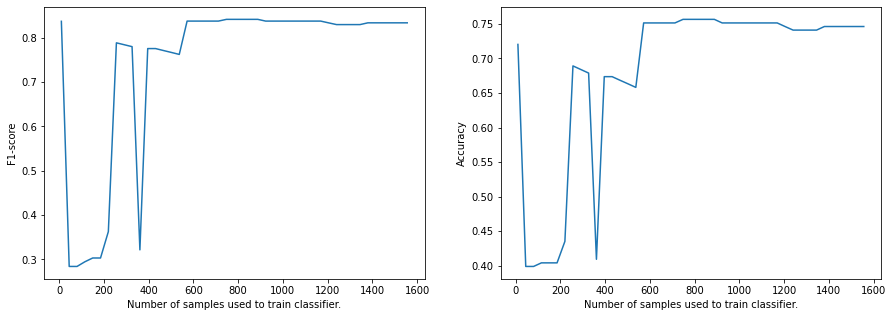
\includegraphics[width=\linewidth]{reports/figures/A1_classification_svc_cluster1.png}
    \caption{Evolution of F1 score and accuracy for the support vector classification in approach 1 (cluster 1).}
    \label{fig:A1_classification_svc_cluster1}
\end{figure*}

\begin{table*}[h]
  \caption{Table of metrics for the support vector classification in approach 1 (cluster 1).}
  \label{tab:A1_classification_svc_cluster1}
  \begin{tabular}{cllllll}
    \toprule
    Number of samples & accuracy & balancedaccuracy & adjusted balanced accuracy & f1 & f1 weighted & matthews\\
    \midrule
       10 & 0.720 & 0.500 & 0.000 & 0.837 & 0.603 & 0.000\\
       45 & 0.399 & 0.583 & 0.165 & 0.284 & 0.339 & 0.229\\
       80 & 0.399 & 0.583 & 0.165 & 0.284 & 0.339 & 0.229\\
      115 & 0.404 & 0.586 & 0.173 & 0.294 & 0.348 & 0.235\\
      150 & 0.404 & 0.581 & 0.161 & 0.303 & 0.352 & 0.212\\
      185 & 0.404 & 0.581 & 0.161 & 0.303 & 0.352 & 0.212\\
      220 & 0.435 & 0.602 & 0.205 & 0.363 & 0.399 & 0.247\\
      256 & 0.689 & 0.597 & 0.195 & 0.789 & 0.683 & 0.202\\
      291 & 0.684 & 0.594 & 0.187 & 0.784 & 0.679 & 0.193\\
      326 & 0.679 & 0.590 & 0.180 & 0.780 & 0.675 & 0.185\\
      361 & 0.409 & 0.579 & 0.157 & 0.321 & 0.365 & 0.197\\
      396 & 0.674 & 0.587 & 0.173 & 0.776 & 0.671 & 0.176\\
      431 & 0.674 & 0.587 & 0.173 & 0.776 & 0.671 & 0.176\\
      466 & 0.668 & 0.583 & 0.166 & 0.771 & 0.666 & 0.168\\
      502 & 0.663 & 0.579 & 0.159 & 0.767 & 0.662 & 0.160\\
      537 & 0.658 & 0.576 & 0.151 & 0.763 & 0.658 & 0.151\\
      572 & 0.751 & 0.640 & 0.281 & 0.838 & 0.734 & 0.324\\
      607 & 0.751 & 0.640 & 0.281 & 0.838 & 0.734 & 0.324\\
      642 & 0.751 & 0.640 & 0.281 & 0.838 & 0.734 & 0.324\\
      677 & 0.751 & 0.640 & 0.281 & 0.838 & 0.734 & 0.324\\
      712 & 0.751 & 0.640 & 0.281 & 0.838 & 0.734 & 0.324\\
      748 & 0.756 & 0.644 & 0.288 & 0.842 & 0.738 & 0.336\\
      783 & 0.756 & 0.644 & 0.288 & 0.842 & 0.738 & 0.336\\
      818 & 0.756 & 0.644 & 0.288 & 0.842 & 0.738 & 0.336\\
      853 & 0.756 & 0.644 & 0.288 & 0.842 & 0.738 & 0.336\\
      888 & 0.756 & 0.644 & 0.288 & 0.842 & 0.738 & 0.336\\
      923 & 0.751 & 0.640 & 0.281 & 0.838 & 0.734 & 0.324\\
      958 & 0.751 & 0.640 & 0.281 & 0.838 & 0.734 & 0.324\\
      994 & 0.751 & 0.640 & 0.281 & 0.838 & 0.734 & 0.324\\
     1029 & 0.751 & 0.640 & 0.281 & 0.838 & 0.734 & 0.324\\
     1064 & 0.751 & 0.640 & 0.281 & 0.838 & 0.734 & 0.324\\
     1099 & 0.751 & 0.640 & 0.281 & 0.838 & 0.734 & 0.324\\
     1134 & 0.751 & 0.640 & 0.281 & 0.838 & 0.734 & 0.324\\
     1169 & 0.751 & 0.640 & 0.281 & 0.838 & 0.734 & 0.324\\
     1204 & 0.746 & 0.637 & 0.274 & 0.834 & 0.730 & 0.312\\
     1240 & 0.741 & 0.633 & 0.267 & 0.830 & 0.725 & 0.301\\
     1275 & 0.741 & 0.633 & 0.267 & 0.830 & 0.725 & 0.301\\
     1310 & 0.741 & 0.633 & 0.267 & 0.830 & 0.725 & 0.301\\
     1345 & 0.741 & 0.633 & 0.267 & 0.830 & 0.725 & 0.301\\
     1380 & 0.746 & 0.637 & 0.274 & 0.834 & 0.730 & 0.312\\
     1415 & 0.746 & 0.637 & 0.274 & 0.834 & 0.730 & 0.312\\
     1450 & 0.746 & 0.637 & 0.274 & 0.834 & 0.730 & 0.312\\
     1486 & 0.746 & 0.637 & 0.274 & 0.834 & 0.730 & 0.312\\
     1521 & 0.746 & 0.637 & 0.274 & 0.834 & 0.730 & 0.312\\
     1556 & 0.746 & 0.637 & 0.274 & 0.834 & 0.730 & 0.312\\
    \bottomrule
    \end{tabular}
\end{table*}

\begin{figure*}[h]
    \centering
    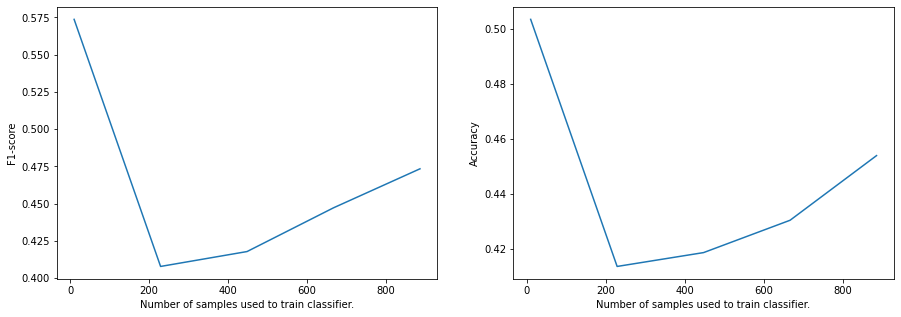
\includegraphics[width=\linewidth]{reports/figures/A1_classification_knn_cluster0.png}
    \caption{Evolution of F1 score and accuracy for the KNN classification in approach 1 (cluster 0).}
    \label{fig:A1_classification_knn_cluster0}
\end{figure*}

\begin{table*}[h]
  \caption{Table of metrics for the KNN classification in approach 1 (cluster 0).}
  \label{tab:A1_classification_knn_cluster0}
  \begin{tabular}{cllllll}
    \toprule
    Number of samples & accuracy & balancedaccuracy & adjusted balanced accuracy & f1 & f1 weighted & matthews\\
    \midrule
       10 & 0.503 & 0.534 & 0.067 & 0.574 & 0.526 & 0.061\\
      229 & 0.414 & 0.518 & 0.036 & 0.408 & 0.411 & 0.036\\
      448 & 0.419 & 0.520 & 0.039 & 0.418 & 0.418 & 0.039\\
      667 & 0.430 & 0.517 & 0.034 & 0.447 & 0.438 & 0.033\\
      886 & 0.454 & 0.542 & 0.084 & 0.473 & 0.462 & 0.081\\
    \bottomrule
    \end{tabular}
\end{table*}

\begin{figure*}[h]
    \centering
    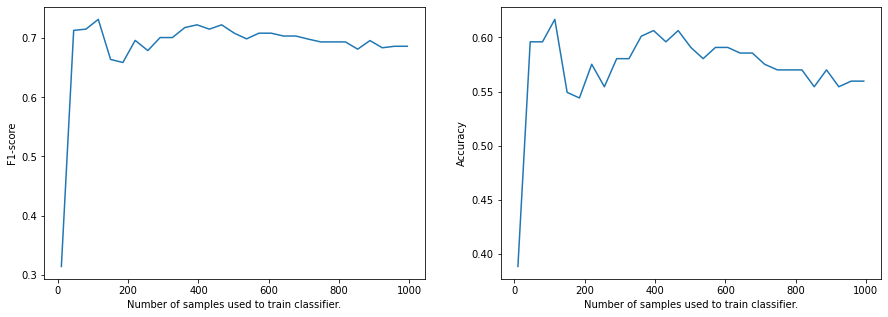
\includegraphics[width=\linewidth]{reports/figures/A1_classification_knn_cluster1.png}
    \caption{Evolution of F1 score and accuracy for the KNN classification in approach 1 (cluster 1).}
    \label{fig:A1_classification_knn_cluster1}
\end{figure*}

\begin{table*}[h]
  \caption{Table of metrics for the KNN classification in approach 1 (cluster 1).}
  \label{tab:A1_classification_knn_cluster1}
  \begin{tabular}{cllllll}
    \toprule
    Number of samples & accuracy & balancedaccuracy & adjusted balanced accuracy & f1 & f1 weighted & matthews\\
    \midrule
        10 & 0.389 & 0.542 & 0.083 & 0.314 & 0.352 & 0.099\\
       45 & 0.596 & 0.516 & 0.031 & 0.713 & 0.602 & 0.030\\
       80 & 0.596 & 0.510 & 0.020 & 0.715 & 0.600 & 0.019\\
      115 & 0.617 & 0.530 & 0.060 & 0.732 & 0.619 & 0.059\\
      150 & 0.549 & 0.495 &-0.011 & 0.664 & 0.566 &-0.010\\
      185 & 0.544 & 0.491 &-0.018 & 0.659 & 0.562 &-0.017\\
      220 & 0.575 & 0.496 &-0.009 & 0.696 & 0.583 &-0.009\\
      256 & 0.554 & 0.475 &-0.049 & 0.679 & 0.565 &-0.047\\
      291 & 0.580 & 0.499 &-0.002 & 0.701 & 0.588 &-0.002\\
      326 & 0.580 & 0.499 &-0.002 & 0.701 & 0.588 &-0.002\\
      361 & 0.601 & 0.519 & 0.038 & 0.718 & 0.606 & 0.037\\
      396 & 0.606 & 0.523 & 0.046 & 0.723 & 0.610 & 0.045\\
      431 & 0.596 & 0.510 & 0.020 & 0.715 & 0.600 & 0.019\\
      466 & 0.606 & 0.523 & 0.046 & 0.723 & 0.610 & 0.045\\
      502 & 0.591 & 0.512 & 0.024 & 0.708 & 0.598 & 0.023\\
      537 & 0.580 & 0.505 & 0.010 & 0.699 & 0.589 & 0.009\\
      572 & 0.591 & 0.512 & 0.024 & 0.708 & 0.598 & 0.023\\
      607 & 0.591 & 0.512 & 0.024 & 0.708 & 0.598 & 0.023\\
      642 & 0.585 & 0.508 & 0.017 & 0.704 & 0.594 & 0.016\\
      677 & 0.585 & 0.508 & 0.017 & 0.704 & 0.594 & 0.016\\
      712 & 0.575 & 0.490 &-0.020 & 0.699 & 0.582 &-0.020\\
      748 & 0.570 & 0.486 &-0.027 & 0.694 & 0.577 &-0.026\\
      783 & 0.570 & 0.486 &-0.027 & 0.694 & 0.577 &-0.026\\
      818 & 0.570 & 0.486 &-0.027 & 0.694 & 0.577 &-0.026\\
      853 & 0.554 & 0.470 &-0.060 & 0.681 & 0.563 &-0.058\\
      888 & 0.570 & 0.481 &-0.039 & 0.696 & 0.576 &-0.038\\
      923 & 0.554 & 0.464 &-0.072 & 0.684 & 0.561 &-0.070\\
      958 & 0.560 & 0.473 &-0.053 & 0.686 & 0.567 &-0.051\\
      994 & 0.560 & 0.473 &-0.053 & 0.686 & 0.567 &-0.051\\
    \bottomrule
    \end{tabular}
\end{table*}

\begin{figure*}[h]
    \centering
    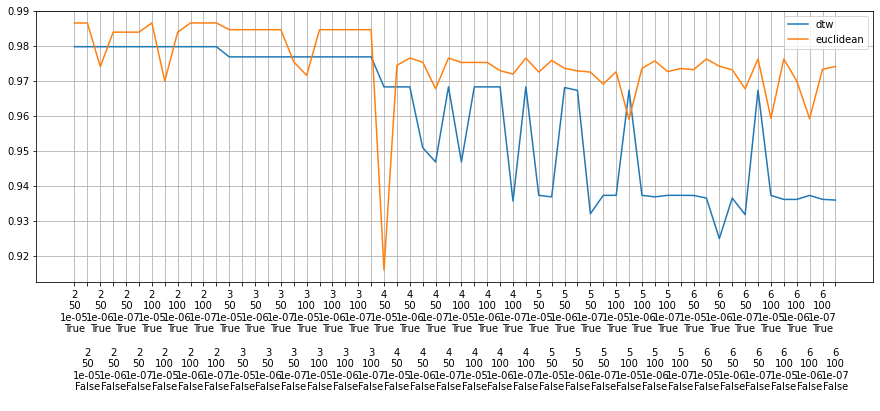
\includegraphics[width=\linewidth]{reports/figures/A2_clustering_german_kmeans.png}
    \caption{Evolution of the silhouette score with the hyperparameter tuning for the time series KMeans clustering in A2. Parameters respectively are number of clusters, max iterations, tolerance, distance metric, inertia. (Please refer to section \ref{sec:results} for explanations on each parameter).}
    \label{fig:A2_clustering_german_kmeans}
\end{figure*}

\begin{figure*}[h]
    \centering
    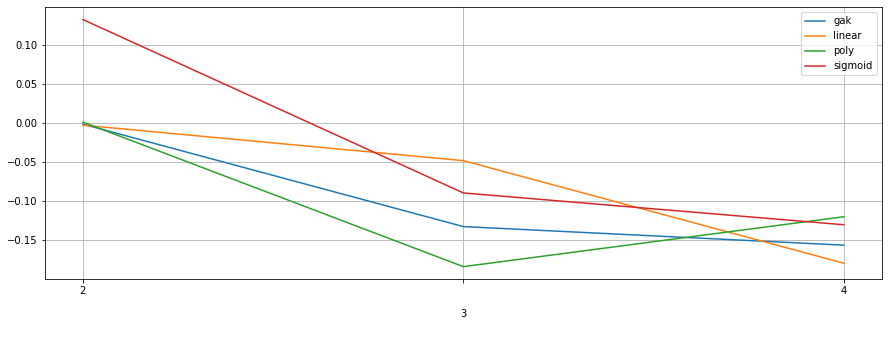
\includegraphics[width=\linewidth]{reports/figures/A2_clustering_math_kernel.png}
    \caption{Evolution of the silhouette score with the hyperparameter tuning for the time series Kernel clustering in A2. Parameters respectively are number of clusters. The different lines indicate the different kernels used for the clustering. (Please refer to section \ref{sec:results} for explanations on each parameter).}
    \label{fig:A2_clustering_math_kernel}
\end{figure*}

\begin{table*}[h]
  \caption{Grid used for finding the best parameter combination for a \emph{Decision Tree Classifier}.}
  \label{tab:grid_dt}
  \begin{tabular}{cl}
    \toprule
    \textbf{Parameter}&\textbf{Values}\\
    \midrule
    $\texttt{min\_samples\_split}$ & $\{2, 5, 10\}$ \\
    $\texttt{min\_samples\_leaf}$ & $\{1, 2, 4\}$ \\
    $\texttt{max\_features}$ & $\{\texttt{auto}, \texttt{sqrt}\}$ \\
    $\texttt{max\_depth}$ & $\{10, 20, 30, 40, 50, 60, 70, 80, 90, 100, 110, \texttt{None}\}$ \\
    \bottomrule
    \end{tabular}
\end{table*}

\begin{table*}[h]
  \caption{Grid used for finding the best parameter combination for a \emph{Random Forest Classifier}.}
  \label{tab:grid_rf}
  \begin{tabular}{cl}
    \toprule
    \textbf{Parameter}&\textbf{Values}\\
    \midrule
    $\texttt{n\_estimators}$ & $\{200, 400, 600, 800, 1000, 1200, 1400, 1600, 1800, 2000\}$\\
    $\texttt{min\_samples\_split}$ & $\{2, 5, 10\}$ \\
    $\texttt{min\_samples\_leaf}$ & $\{1, 2, 4\}$ \\
    $\texttt{max\_features}$ & $\{\texttt{auto}, \texttt{sqrt}\}$ \\
    $\texttt{max\_depth}$ & $\{10, 20, 30, 40, 50, 60, 70, 80, 90, 100, 110, \texttt{None}\}$ \\
    $\texttt{bootstrap}$ & $\{\texttt{True}, \texttt{False}\}$
    \bottomrule
    \end{tabular}
\end{table*}

\begin{table*}[h]
  \caption{Best parameters combination for a \emph{Decision Tree Classifier} in \emph{Experiment 1}.}
  \label{tab:dc_1}
  \begin{tabular}{cl}
    \toprule
    \textbf{Parameter}&\textbf{Value}\\
    \midrule
    $\texttt{min\_samples\_split}$ & $5$ \\
    $\texttt{min\_samples\_leaf}$ & $1$ \\
    $\texttt{max\_features}$ & $\texttt{auto}$ \\
    $\texttt{max\_depth}$ & $40$ \\
    \bottomrule
    \end{tabular}
\end{table*}

\begin{table*}[h]
  \caption{Best parameters combination for a \emph{Decision Tree Classifier} in \emph{Experiment 2}.}
  \label{tab:dc_2}
  \begin{tabular}{cl}
    \toprule
    \textbf{Parameter}&\textbf{Value}\\
    \midrule
    $\texttt{min\_samples\_split}$ & $2$ \\
    $\texttt{min\_samples\_leaf}$ & $1$ \\
    $\texttt{max\_features}$ & $\texttt{sqrt}$ \\
    $\texttt{max\_depth}$ & $80$ \\
    \bottomrule
    \end{tabular}
\end{table*}

\begin{table*}[h]
  \caption{Best parameters combination for a \emph{Random Forest Classifier} in \emph{Experiment 1}.}
  \label{tab:rf_1}
  \begin{tabular}{cl}
    \toprule
    \textbf{Parameter}&\textbf{Value}\\
    \midrule
    $\texttt{n\_estimators}$ & $1400$\\
    $\texttt{min\_samples\_split}$ & $10$ \\
    $\texttt{min\_samples\_leaf}$ & $1$ \\
    $\texttt{max\_features}$ & $\texttt{auto}$ \\
    $\texttt{max\_depth}$ & $110$ \\
    $\texttt{bootstrap}$ & $\texttt{False}$ \\
    \bottomrule
    \end{tabular}
\end{table*}

\begin{table*}[h]
  \caption{Best parameters combination for a \emph{Random Forest Classifier} in \emph{Experiment 2}.}
  \label{tab:rf_2}
  \begin{tabular}{cl}
    \toprule
    \textbf{Parameter}&\textbf{Value}\\
    \midrule
    $\texttt{n\_estimators}$ & $400$\\
    $\texttt{min\_samples\_split}$ & $2$ \\
    $\texttt{min\_samples\_leaf}$ & $1$ \\
    $\texttt{max\_features}$ & $\texttt{auto}$ \\
    $\texttt{max\_depth}$ & $70$ \\
    $\texttt{bootstrap}$ & $\texttt{False}$ \\
    \bottomrule
    \end{tabular}
\end{table*}

\begin{table*}[h]
  \caption{\textbf{Accuracy}, \textbf{balanced accuracy}, \textbf{adjusted balanced accuracy}, \textbf{F1 score}, \textbf{weighted F1 score} and \textbf{Matthew's coefficient} for the \emph{Random Forest Classifier} trained in \emph{Experiment 2}.}
  \label{tab:rf_2_table_results}
  \begin{tabular}{cllllll}
    \toprule
    \textbf{Samples}&\textbf{Accuracy}&\textbf{Balanced Accuracy}&\textbf{Adj. Balanced Accuracy}&\textbf{F1}&\textbf{Weighted F1}&\textbf{Matthew's coeff.}\\
    \midrule
    $10$ & $0.592$ & $0.557$ & $0.114$ & $0.695$ & $0.613$ & $0.103$\\
    $168$ & $0.589$ & $0.568$ & $0.136$ & $0.688$ & $0.612$ & $0.121$\\
    $327$ & $0.569$ & $0.566$ & $0.132$ & $0.662$ & $0.595$ & $0.117$\\
    $486$ & $0.583$ & $0.564$ & $0.129$ & $0.681$ & $0.607$ & $0.114$\\
    $644$ & $0.567$ & $0.560$ & $0.119$ & $0.662$ & $0.592$ & $0.106$\\
    $803$ & $0.580$ & $0.560$ & $0.120$ & $0.679$ & $0.604$ & $0.107$\\
    $962$ & $0.561$ & $0.550$ & $0.100$ & $0.658$ & $0.587$ & $0.089$\\
    \bottomrule
    \end{tabular}
\end{table*}

\begin{table*}[h]
  \caption{\textbf{Accuracy}, \textbf{balanced accuracy}, \textbf{adjusted balanced accuracy}, \textbf{F1 score}, \textbf{weighted F1 score} and \textbf{Matthew's coefficient} for the \emph{Decision Tree Classifier} trained in \emph{Experiment 1}.}
  \label{tab:dc_1_table_results}
  \begin{tabular}{cllllll}
    \toprule
    \textbf{Samples}&\textbf{Accuracy}&\textbf{Balanced Accuracy}&\textbf{Adj. Balanced Accuracy}&\textbf{F1}&\textbf{Weighted F1}&\textbf{Matthew's coeff.}\\
    \midrule
    $10$ & $0.540$ & $0.544$ & $0.089$ & $0.632$ & $0.567$ & $0.078$\\
    $168$ & $0.880$ & $0.895$ & $0.789$ & $0.914$ & $0.885$ & $0.732$\\
    $327$ & $0.965$ & $0.969$ & $0.939$ & $0.976$ & $0.966$ & $0.914$\\
    $486$ & $0.875$ & $0.880$ & $0.759$ & $0.911$ & $0.879$ & $0.710$\\
    $644$ & $0.999$ & $0.999$ & $0.999$ & $0.999$ & $0.999$ & $0.998$\\
    $803$ & $0.960$ & $0.959$ & $0.918$ & $0.972$ & $0.960$ & $0.900$\\
    $962$ & $1.000$ & $1.000$ & $1.000$ & $1.000$ & $1.000$ & $1.000$\\
    \bottomrule
    \end{tabular}
\end{table*}

\begin{table*}[h]
  \caption{\textbf{Accuracy}, \textbf{balanced accuracy}, \textbf{adjusted balanced accuracy}, \textbf{F1 score}, \textbf{weighted F1 score} and \textbf{Matthew's coefficient} for the \emph{Decision Tree Classifier} trained in \emph{Experiment 2}.}
  \label{tab:dc_2_table_results}
  \begin{tabular}{cllllll}
    \toprule
    \textbf{Samples}&\textbf{Accuracy}&\textbf{Balanced Accuracy}&\textbf{Adj. Balanced Accuracy}&\textbf{F1}&\textbf{Weighted F1}&\textbf{Matthew's coeff.}\\
    \midrule
    $10$ & $0.560$ & $0.545$ & $0.089$ & $0.660$ & $0.586$ & $0.079$\\
    $168$ & $0.573$ & $0.558$ & $0.116$ & $0.671$ & $0.598$ & $0.103$\\
    $327$ & $0.569$ & $0.557$ & $0.113$ & $0.666$ & $0.594$ & $0.100$\\
    $486$ & $0.562$ & $0.545$ & $0.091$ & $0.661$ & $0.587$ & $0.080$\\
    $644$ & $0.553$ & $0.543$ & $0.086$ & $0.650$ & $0.579$ & $0.076$\\
    $803$ & $0.572$ & $0.559$ & $0.119$ & $0.668$ & $0.597$ & $0.105$\\
    $962$ & $0.550$ & $0.534$ & $0.068$ & $0.651$ & $0.576$ & $0.060$\\
    \bottomrule
    \end{tabular}
\end{table*}



\begin{figure*}[h]
    \centering
    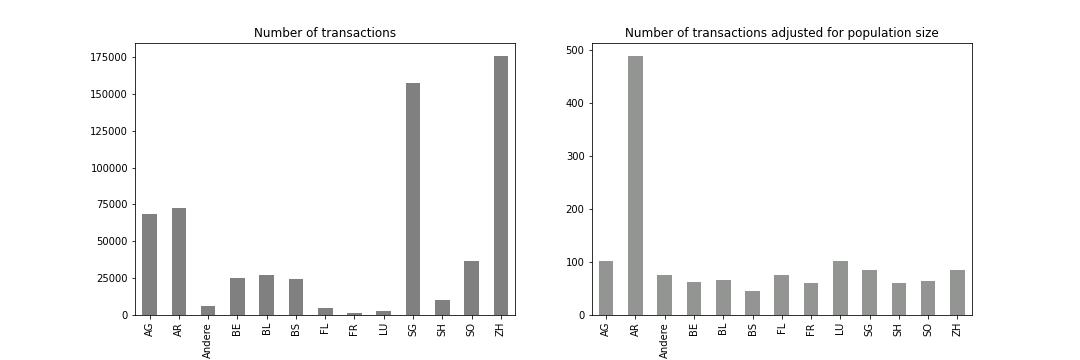
\includegraphics[width=\linewidth]{reports/figures/cantonal_representation.jpg}
    \caption{(Left) Number of transactions per canton. (Right) Number of transactions per canton capita.}
    \label{fig:cantonal_representation}
\end{figure*}

\begin{figure*}[h]
    \centering
    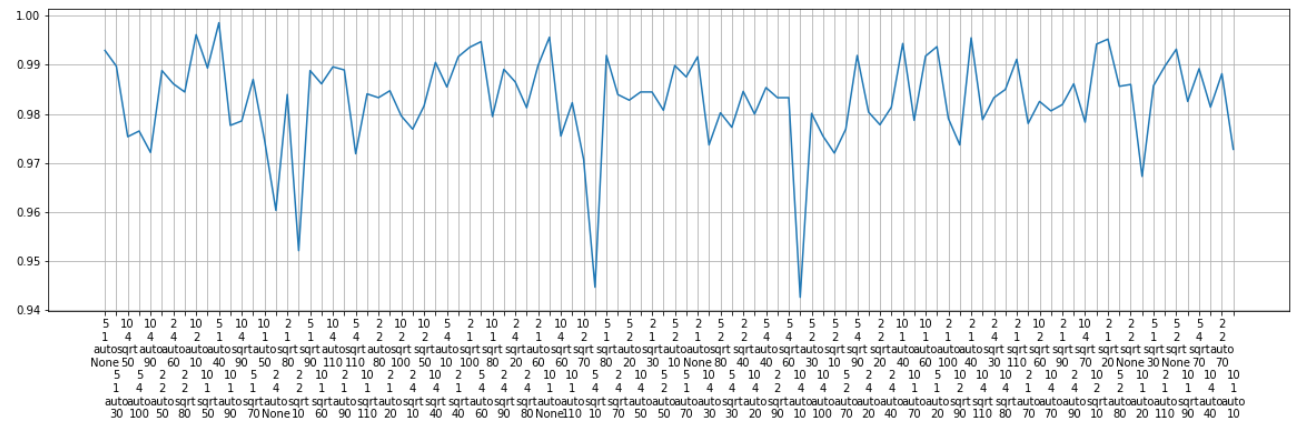
\includegraphics[width=\linewidth]{reports/figures/decision_tree_1.png}
    \caption{Hyperparameter tunning of a \emph{Decision Tree Classifier} in Experiment 1.}
    \label{fig:hyp_decision_1}
\end{figure*}

\begin{figure*}[h]
    \centering
    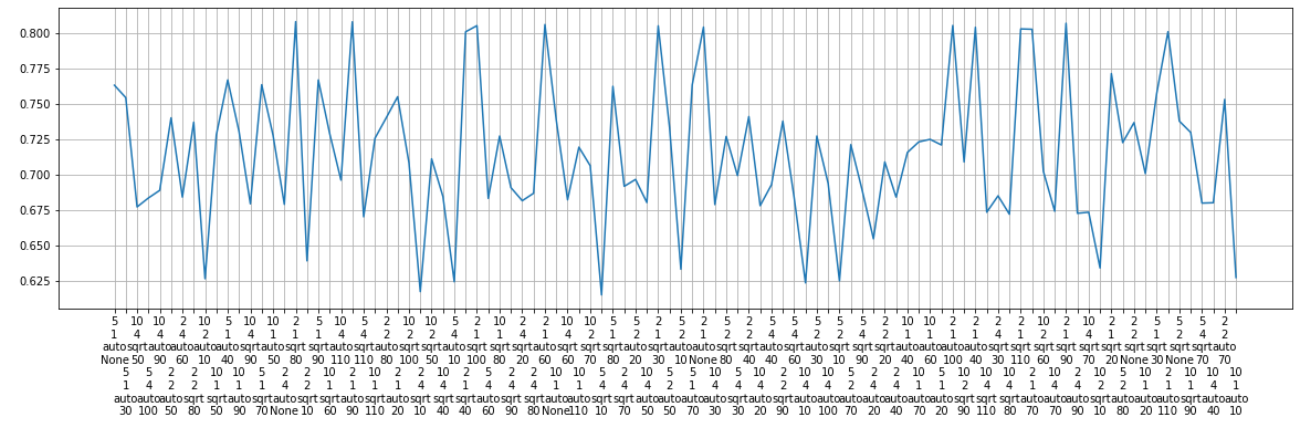
\includegraphics[width=\linewidth]{reports/figures/decision_tree_2.png}
    \caption{Hyperparameter tunning of a \emph{Decision Tree Classifier} in Experiment 2.}
    \label{fig:hyp_decision_2}
\end{figure*}

\begin{figure*}[h]
    \centering
    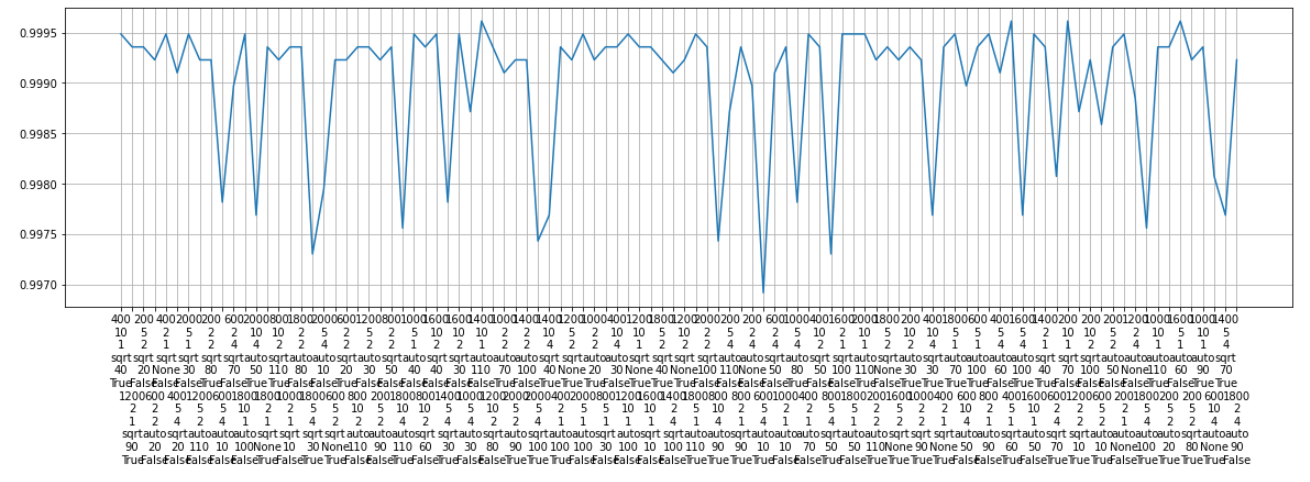
\includegraphics[width=\linewidth]{reports/figures/random_forest_1.png}
    \caption{Hyperparameter tunning of a \emph{Random Forest Classifier} in Experiment 1.}
    \label{fig:hyp_forest_1}
\end{figure*}

\begin{figure*}[h]
    \centering
    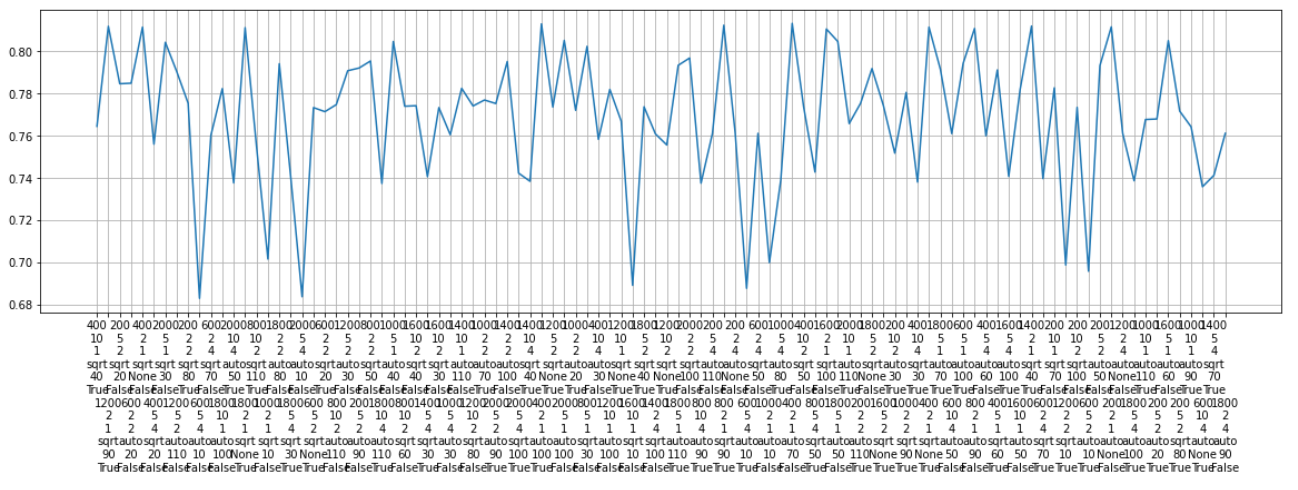
\includegraphics[width=\linewidth]{reports/figures/random_forest_2.png}
    \caption{Hyperparameter tunning of a \emph{Random Forest Classifier} in Experiment 2.}
    \label{fig:hyp_forest_2}
\end{figure*}

 \begin{figure*}[h]
     \centering
     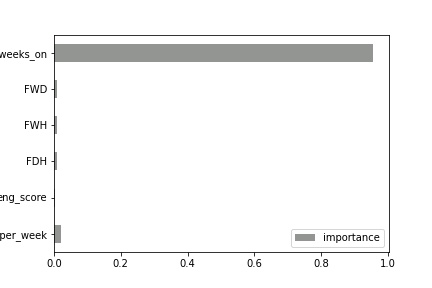
\includegraphics[width=0.5\linewidth]{reports/figures/feature_importance_dc_1.jpg}
     \caption{Bar chart of the \emph{feature importance} of the \emph{Decision Tree Classifier} trained in \emph{Experiment 1}.}
     \label{fig:fi_dc_1}
 \end{figure*}
 
 \begin{figure*}[h]
     \centering
     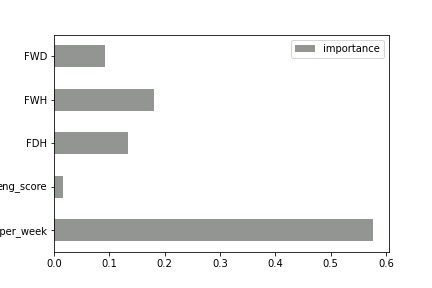
\includegraphics[width=0.5\linewidth]{reports/figures/feature_importance_dc_2.jpg}
     \caption{Bar chart of the \emph{feature importance} of the \emph{Decision Tree Classifier} trained in \emph{Experiment 2}.}
     \label{fig:fi_dc_2}
 \end{figure*}

 \begin{figure*}[h]
     \centering
     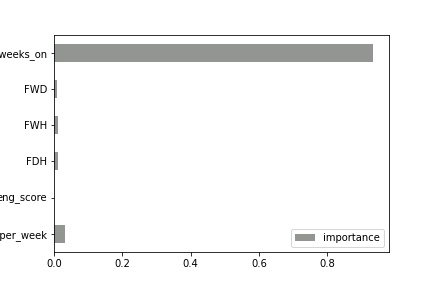
\includegraphics[width=0.5\linewidth]{reports/figures/feature_importance_rf_1.jpg}
     \caption{Bar chart of the \emph{feature importance} of the \emph{Random Forest Classifier} trained in \emph{Experiment 1}.}
     \label{fig:fi_rf_1}
 \end{figure*}
 
 \begin{figure*}[h]
     \centering
     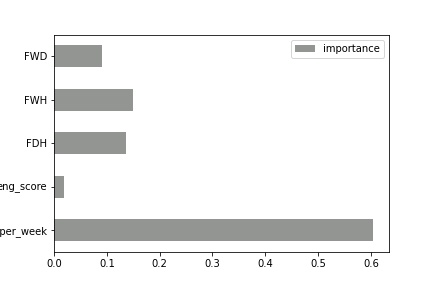
\includegraphics[width=0.5\linewidth]{reports/figures/feature_importance_rf_2.jpg}
     \caption{Bar chart of the \emph{feature importance} of the \emph{Random Forest Classifier} trained in \emph{Experiment 2}.}
     \label{fig:fi_rf_2}
 \end{figure*}
 
  \begin{figure*}[h]
     \centering
     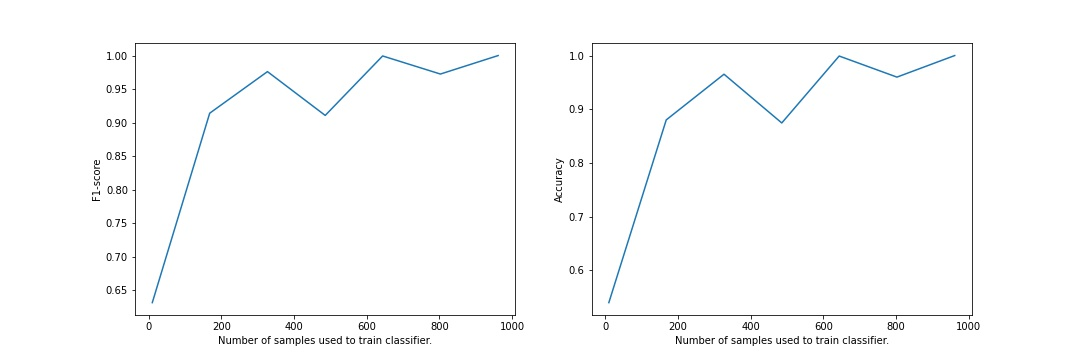
\includegraphics[width=\linewidth]{reports/figures/results_dc_1.jpg}
     \caption{\emph{Accuracy} and \emph{F1-score} against number of samples of the \emph{Decision Tree Classifier} trained in \emph{Experiment 1}.}
     \label{fig:results_dt_1}
 \end{figure*}
 
  \begin{figure*}[h]
     \centering
     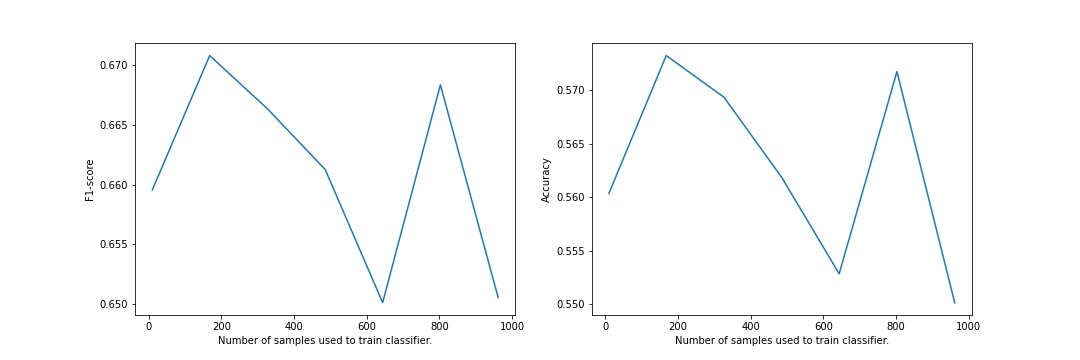
\includegraphics[width=\linewidth]{reports/figures/results_dc_2.jpg}
     \caption{\emph{Accuracy} and \emph{F1-score} against number of samples of the \emph{Decision Tree Classifier} trained in \emph{Experiment 2}.}
     \label{fig:results_dt_2}
 \end{figure*}








\end{document}
\endinput
%%
%% End of file `sample-sigplan.tex'.
